%%%%%%%%%%%%%%%%%%%%%%%%%%%%%%%%%%%%%%%%%%%%%%%%%%%
%% LaTeX book template                           %%
%% Author:  Amber Jain (http://amberj.devio.us/) %%
%% License: ISC license                          %%
%%%%%%%%%%%%%%%%%%%%%%%%%%%%%%%%%%%%%%%%%%%%%%%%%%%

\documentclass[a5paper,11pt]{book}
\usepackage[T1]{fontenc}
\usepackage[utf8]{inputenc}
\usepackage{lmodern}
\usepackage{pifont,kantlipsum}
\usepackage{subfig}
\usepackage{float}
\newcommand*{\altasterism}{\vspace*{1em plus .5em minus .5em}\noindent\hspace*{\fill}\ding{104}\hspace*{\fill}}
\DeclareSymbolFont{extraup}{U}{zavm}{m}{n}
\DeclareMathSymbol{\varheart}{\mathalpha}{extraup}{86}
%%%%%%%%%%%%%%%%%%%%%%%%%%%%%%%%%%%%%%%%%%%%%%%%%%%%%%%%%
% Source: http://en.wikibooks.org/wiki/LaTeX/Hyperlinks %
%%%%%%%%%%%%%%%%%%%%%%%%%%%%%%%%%%%%%%%%%%%%%%%%%%%%%%%%%
\usepackage{hyperref}
\usepackage{graphicx}
\usepackage[english, norsk]{babel}
\usepackage{url,verse}


%%%%%%%%%%%%%%%%%%%%%%%%%%%%%%%%%%%%%%%%%%%%%%%%%%%%%%%%%%%%%%%%%%%%%%%%%%%%%%%%
% 'dedication' environment: To add a dedication paragraph at the start of book %
% Source: http://www.tug.org/pipermail/texhax/2010-June/015184.html            %
%%%%%%%%%%%%%%%%%%%%%%%%%%%%%%%%%%%%%%%%%%%%%%%%%%%%%%%%%%%%%%%%%%%%%%%%%%%%%%%%
\newenvironment{dedication}
{
   \cleardoublepage
   \thispagestyle{empty}
   \vspace*{\stretch{1}}
   \hfill
   \begin{minipage}[t]{0.66\textwidth}
   \raggedright
}
{
   \end{minipage}
   \vspace*{\stretch{3}}
   \clearpage
}

%%%%%%%%%%%%%%%%%%%%%%%%%%%%%%%%%%%%%%%%%%%%%%%%
% Chapter quote at the start of chapter        %
% Source: http://tex.stackexchange.com/a/53380 %
%%%%%%%%%%%%%%%%%%%%%%%%%%%%%%%%%%%%%%%%%%%%%%%%
\makeatletter
\renewcommand{\@chapapp}{}% Not necessary...
\newenvironment{chapquote}[2][2em]
  {\setlength{\@tempdima}{#1}%
   \def\chapquote@author{#2}%
   \parshape 1 \@tempdima \dimexpr\textwidth-2\@tempdima\relax%
   \itshape}
  {\par\normalfont\hfill--\ \chapquote@author\hspace*{\@tempdima}\par\bigskip}
\makeatother

%%%%%%%%%%%%%%%%%%%%%%%%%%%%%%%%%%%%%%%%%%%%%%%%%%%
% First page of book which contains 'stuff' like: %
%  - Book title, subtitle                         %
%  - Book author name                             %
%%%%%%%%%%%%%%%%%%%%%%%%%%%%%%%%%%%%%%%%%%%%%%%%%%%

% Book's title and subtitle
\title{\Huge \textbf{Lisbeths bok}}
% Author
\author{Tekst: Jon, Simone, Ane, Tor Håkon, Oline og Helene,\\ Øivind og Ida\\ Illustrasjoner: Jon, Helene og Oline}

%{\textsc{Ane, Jon, Tor Håkon, Helene, Ulrik og Agnes}}


\begin{document}

\frontmatter
\maketitle

%%%%%%%%%%%%%%%%%%%%%%%%%%%%%%%%%%%%%%%%%%%%%%%%%%%%%%%%%%%%%%%
% Add a dedication paragraph to dedicate your book to someone %
%%%%%%%%%%%%%%%%%%%%%%%%%%%%%%%%%%%%%%%%%%%%%%%%%%%%%%%%%%%%%%%
\begin{dedication}
Til mamma, mormor, og farmor Lisbeth
\end{dedication}

%%%%%%%%%%%%%%%%%%%%%%%%%%%%%%%%%%%%%%%%%%%%%%%%%%%%%%%%%%%%%%%%%%%%%%%%
% Auto-generated table of contents, list of figures and list of tables %
%%%%%%%%%%%%%%%%%%%%%%%%%%%%%%%%%%%%%%%%%%%%%%%%%%%%%%%%%%%%%%%%%%%%%%%%
\tableofcontents
\mainmatter


%%%%%%%%%%%
% Preface %
%%%%%%%%%%%
\chapter*{Forord}
\renewcommand{\baselinestretch}{1.5} 
I anledning at du har fylt 70 år har vi laget denne boken. Det er en samling med historier og bilder om deg, noen fra fantasien og andre fra virkeligheten.\\
Vi håper du setter pris på den og ønsker deg en fabelaktig feiring!\\
Håper boken kan være et påskudd til å få deg til å skrive ned historier om familien og Dalsnes, som alle kan ha glede av.


\begin{flushright}
\textit{Klemmer fra\\
Ane, Jon, Tor Håkon, Helene, Ulrik og Agnes}
\end{flushright}
\newpage
%%%%%%%%%%%%%%%%%%%%%%%%%%%%%%%%%%%%
% Give credit where credit is due. %
% Say thanks!                      %
%%%%%%%%%%%%%%%%%%%%%%%%%%%%%%%%%%%%
 
\section*{Takk}
Takk til Tor Håkon og Oline for timer med skriving av historier! Det har vært veldig gøy å være med på, og å få oppleve fantasien og skrivegleden dere har. Takk til Helene og Oline for flotte illustrasjoner. Takk til Odd for hjelp til å finne fram Lisbeths musikalske karriere.\\
\newline
Takk for fine historier Simone, Ida og Øivind!\\
\newline
%%%%%%%%%%%%%%%%
% NEW CHAPTER! %
%%%%%%%%%%%%%%%%
\chapter{Lisbeth fra Dalsnes}

\begin{chapquote}{Herbjørg Wassmo}
``Noen ganger koster det mer å være feig enn å hoppe uti og se hva som skjer.''
\end{chapquote}

\section{Dalsnes}
\begin{figure}[H]
    \centering
    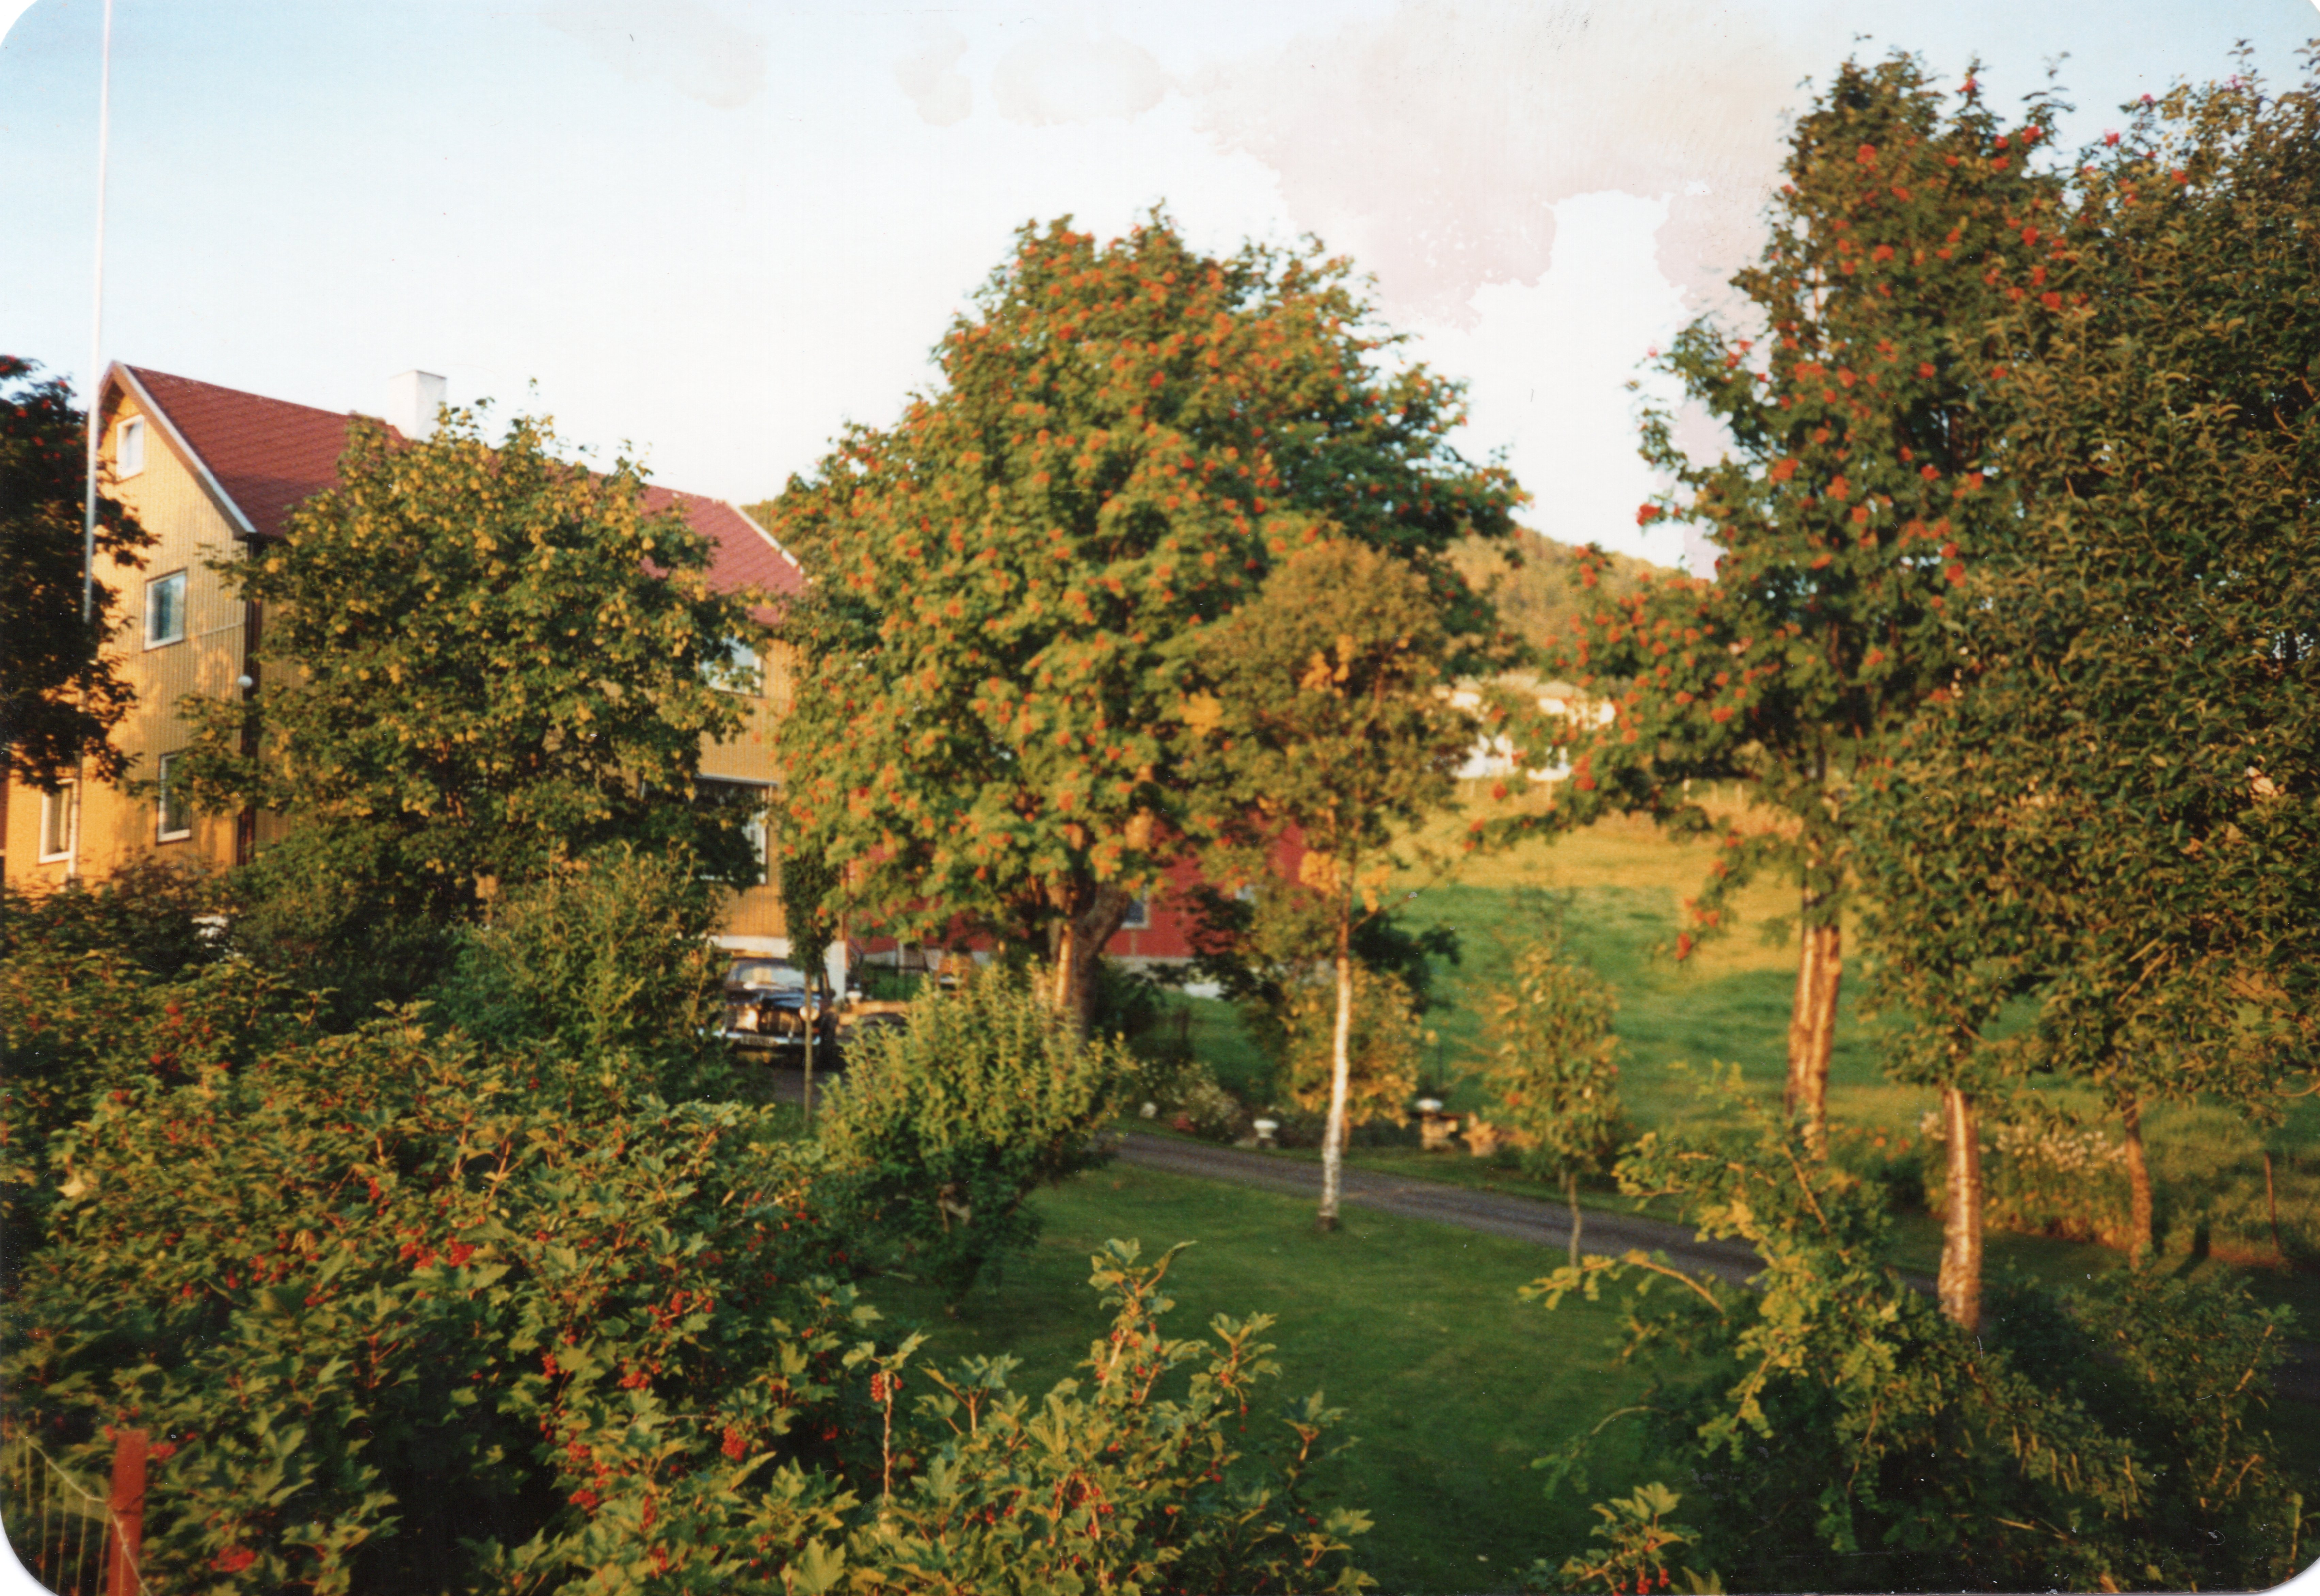
\includegraphics[width=1\textwidth]{illustrasjoner/Dalsnes.jpg}
   \label{Dalsnes}
\end{figure}
Barndomshjemmet på Dalsnes i Kvæfjord, fra Mor Oline's side.

\section{Søsknene Fredriksen}
%Bilder av alle søsknene
\begin{figure}[H]
    \centering
    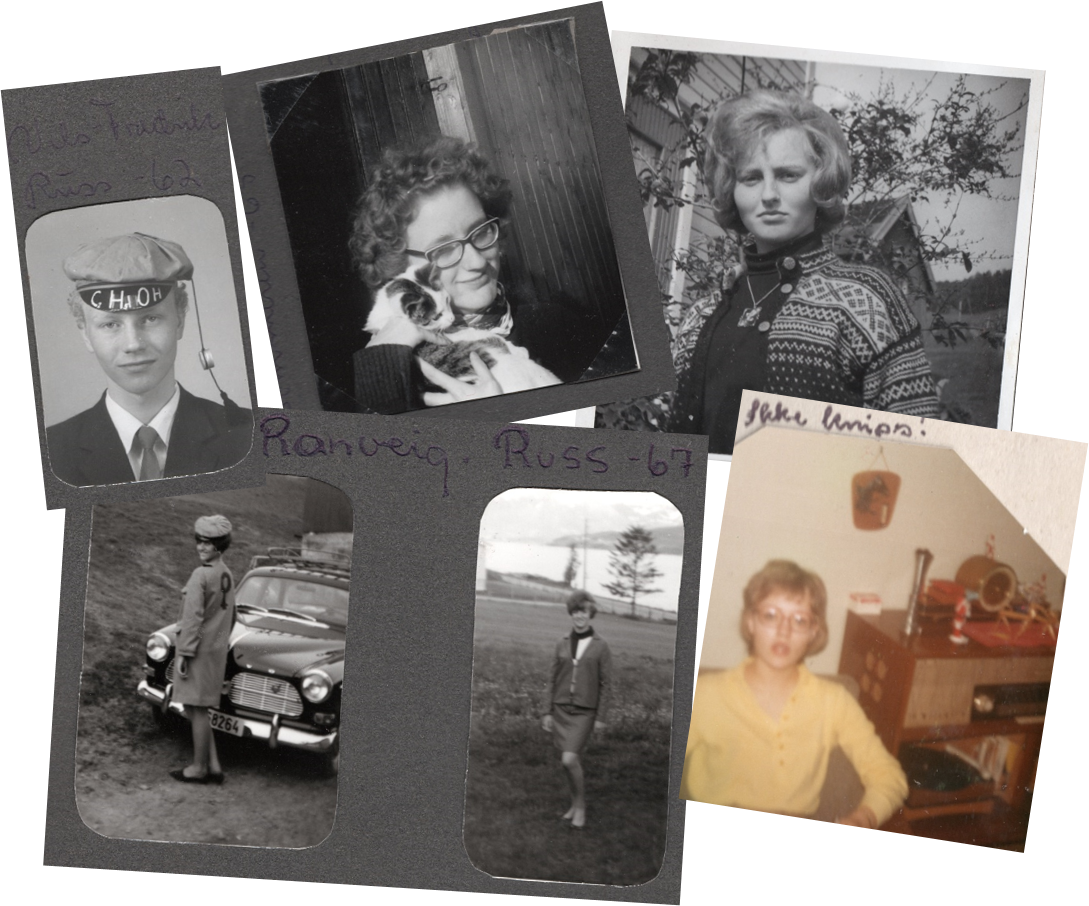
\includegraphics[width=1\textwidth]{illustrasjoner/sosken.png}
   \label{sosken}
\end{figure}

Du var midtpunktet i en søskenflokk på fem. Nils Fredrik kom først. Deretter Britt Margit, hvor Oline ble syk under graviditeten. Det førte visstnok til at du ble flaska opp på feit og god kost og ble en kraftplugg. Du kom til 8. april 1949. Ranveig og Kristin fulgte på. Du hadde dermed fra ung alder ansvar for både storesøster Britt og småsøstrene. 

\section{Forfatterskap}
\begin{figure}[H]
    \centering
    
\includegraphics[scale=0.5]{illustrasjoner/noseb.png}
   \label{Noseb}
\end{figure}

Graham Clifford og Lisbeth Dalsnes\\
\textit{Hjelpetjenesten - reform eller retrett? En evaluering av hjelpetjenesteprosjektet i Saupstad bydel}\\
Trondheim (80 s)\\
1992\\
ISSN 0802-6319
\section{Platekarriere}

\begin{figure}[H]
    \centering
    \includegraphics[width=0.97\textwidth]{illustrasjoner/platekarriere.jpg}
   \label{Plater}
\end{figure}
Du har hatt en liten karriere som plateartist også. To plater har du bidratt på: \textit{Palestina} (1975) med Rødt kor på sangene \textit{Fedayine} og \textit{Biladi}, og på Sverre Kjeldsberg \textit{Etter mørketid} (1978) på \textit{Et fritt Eritrea}. Etter det er det sannsynlig at du var for opptatt med unger og jobb til å ta den musikalske karriere videre.
\bigskip
\newpage
\section{Sangtekstforfatterskapet}
\begin{figure}[H]
    \centering
    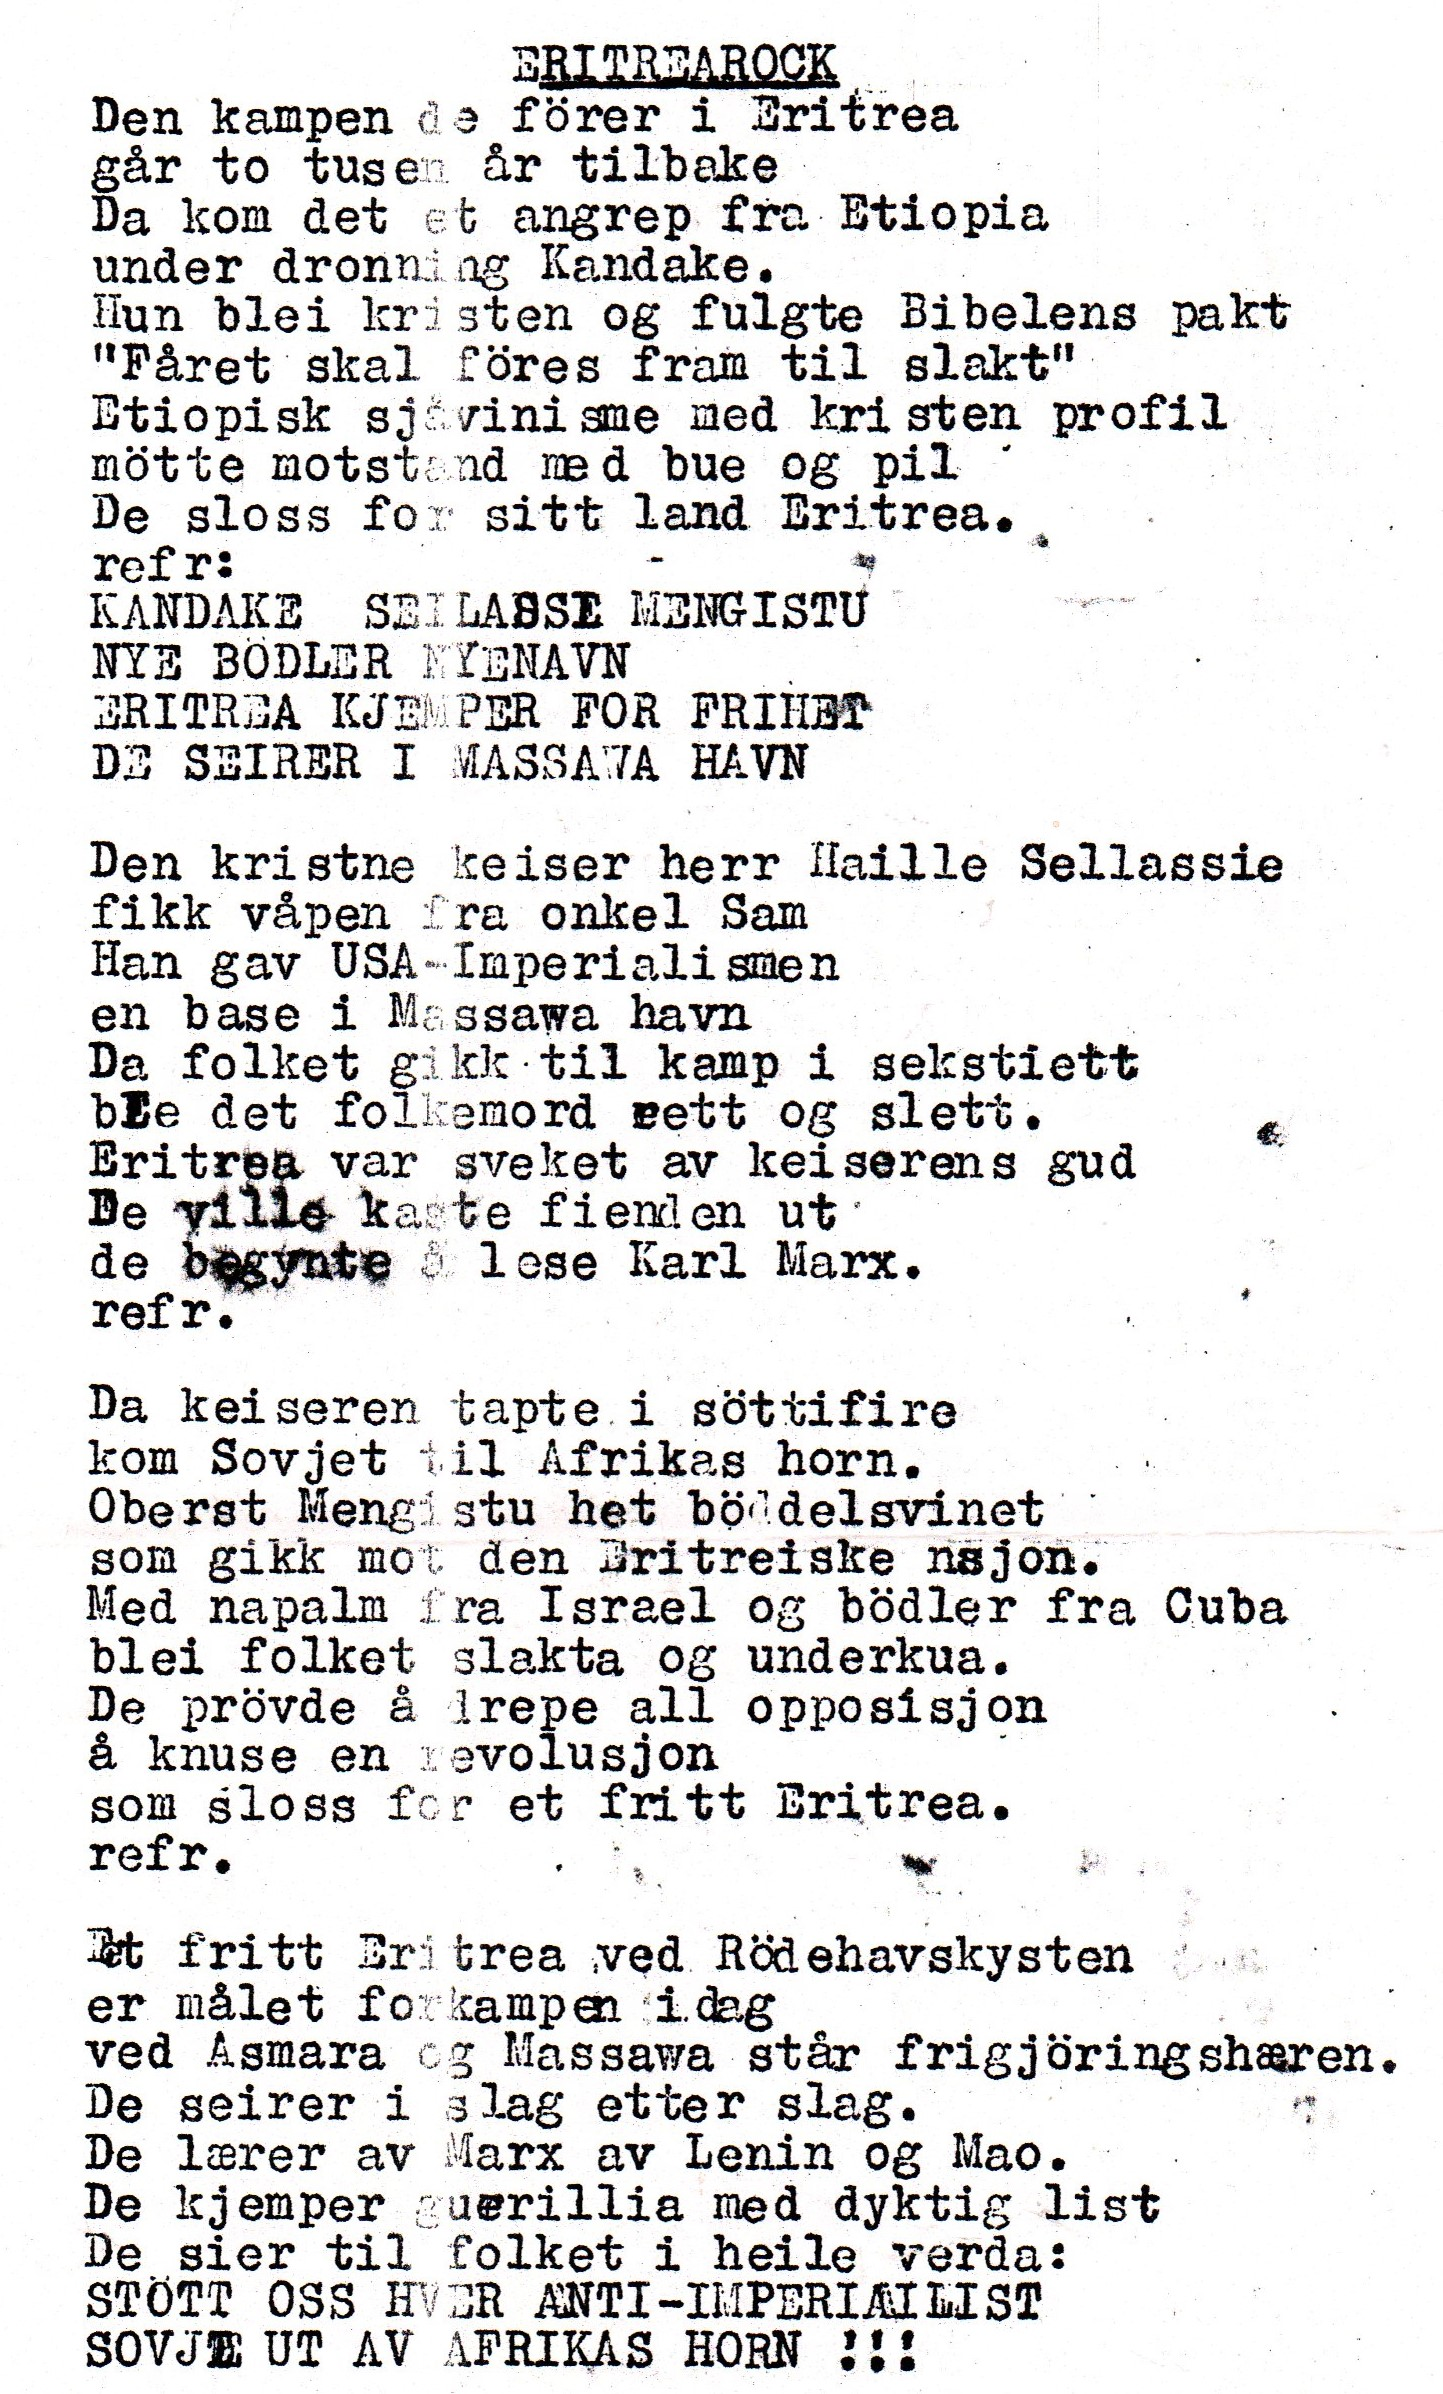
\includegraphics[scale=0.5]{illustrasjoner/Eritrearock.jpg}
   \label{Eritrearock}
\end{figure}

Sangtekstforfatter-karrieren har du klart å holde gående i 40 år, og vi håper på flere i tiårene som kommer! Her gjengis bare et lite utdrag fra kolleksjonen.

\begin{figure}[H]
    \centering
    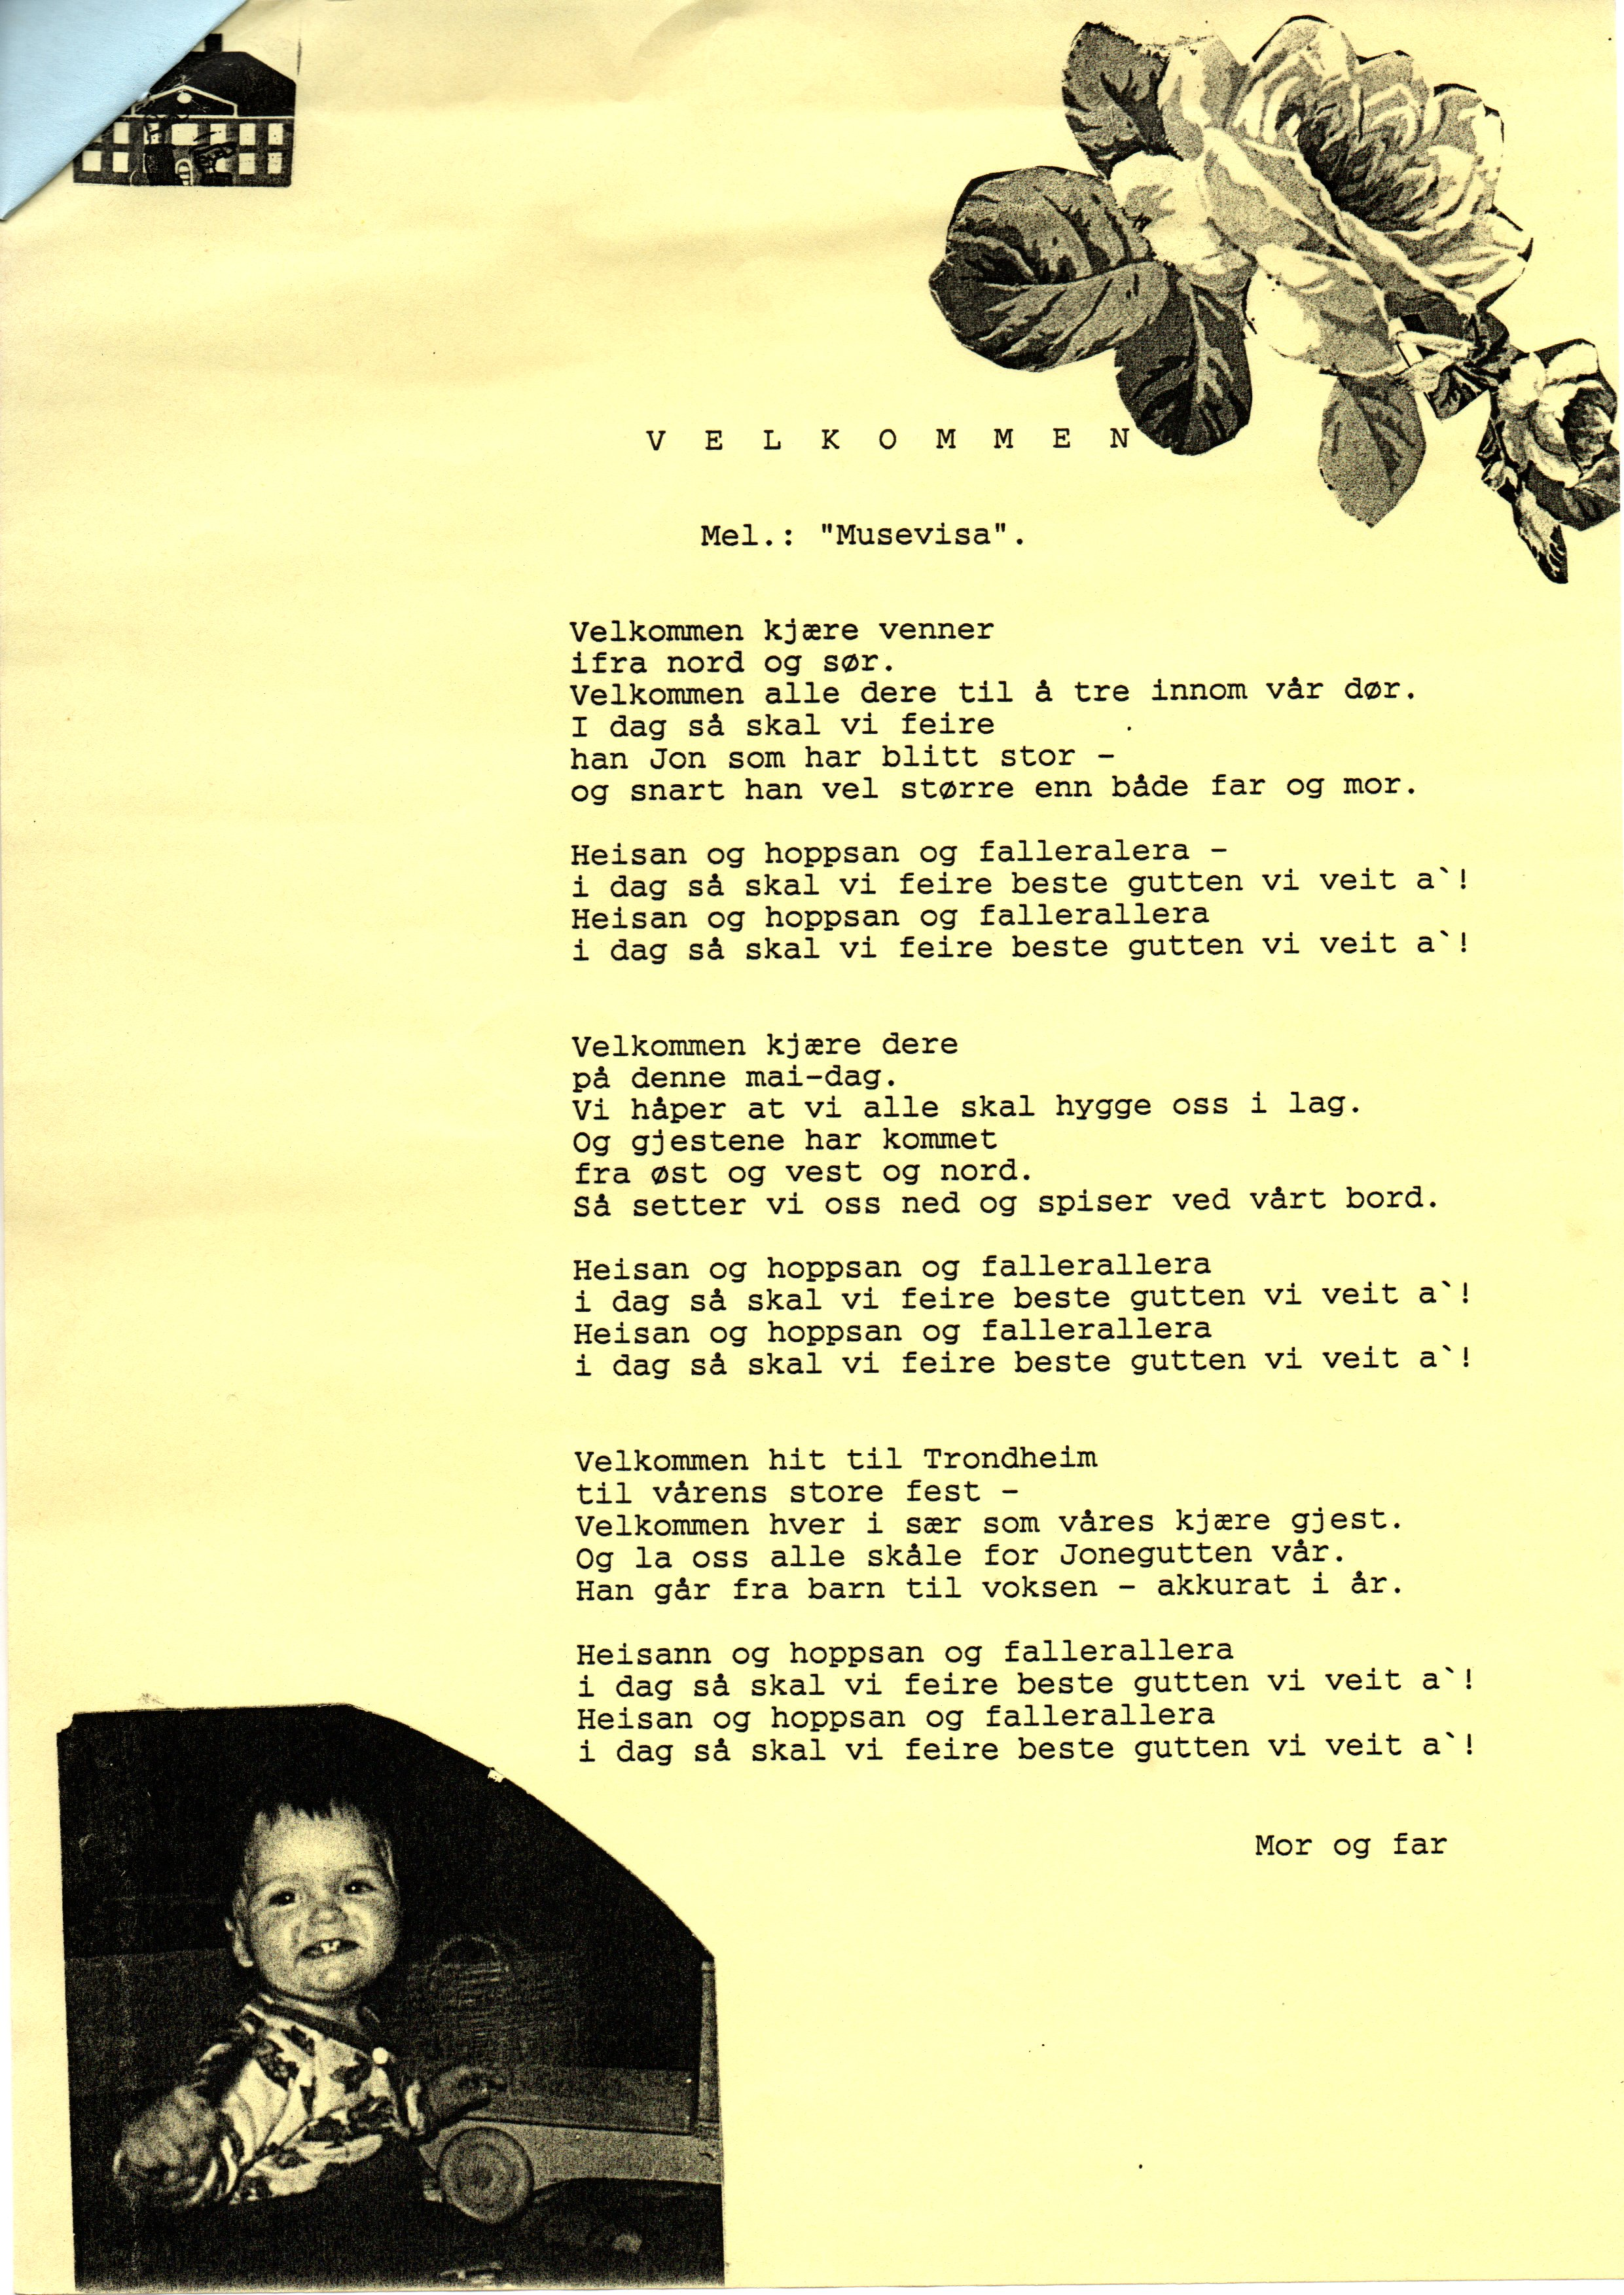
\includegraphics[scale=0.35]{illustrasjoner/jon1.jpg}
   \label{Jon1}
\end{figure}
\begin{figure}[H]
    \centering
    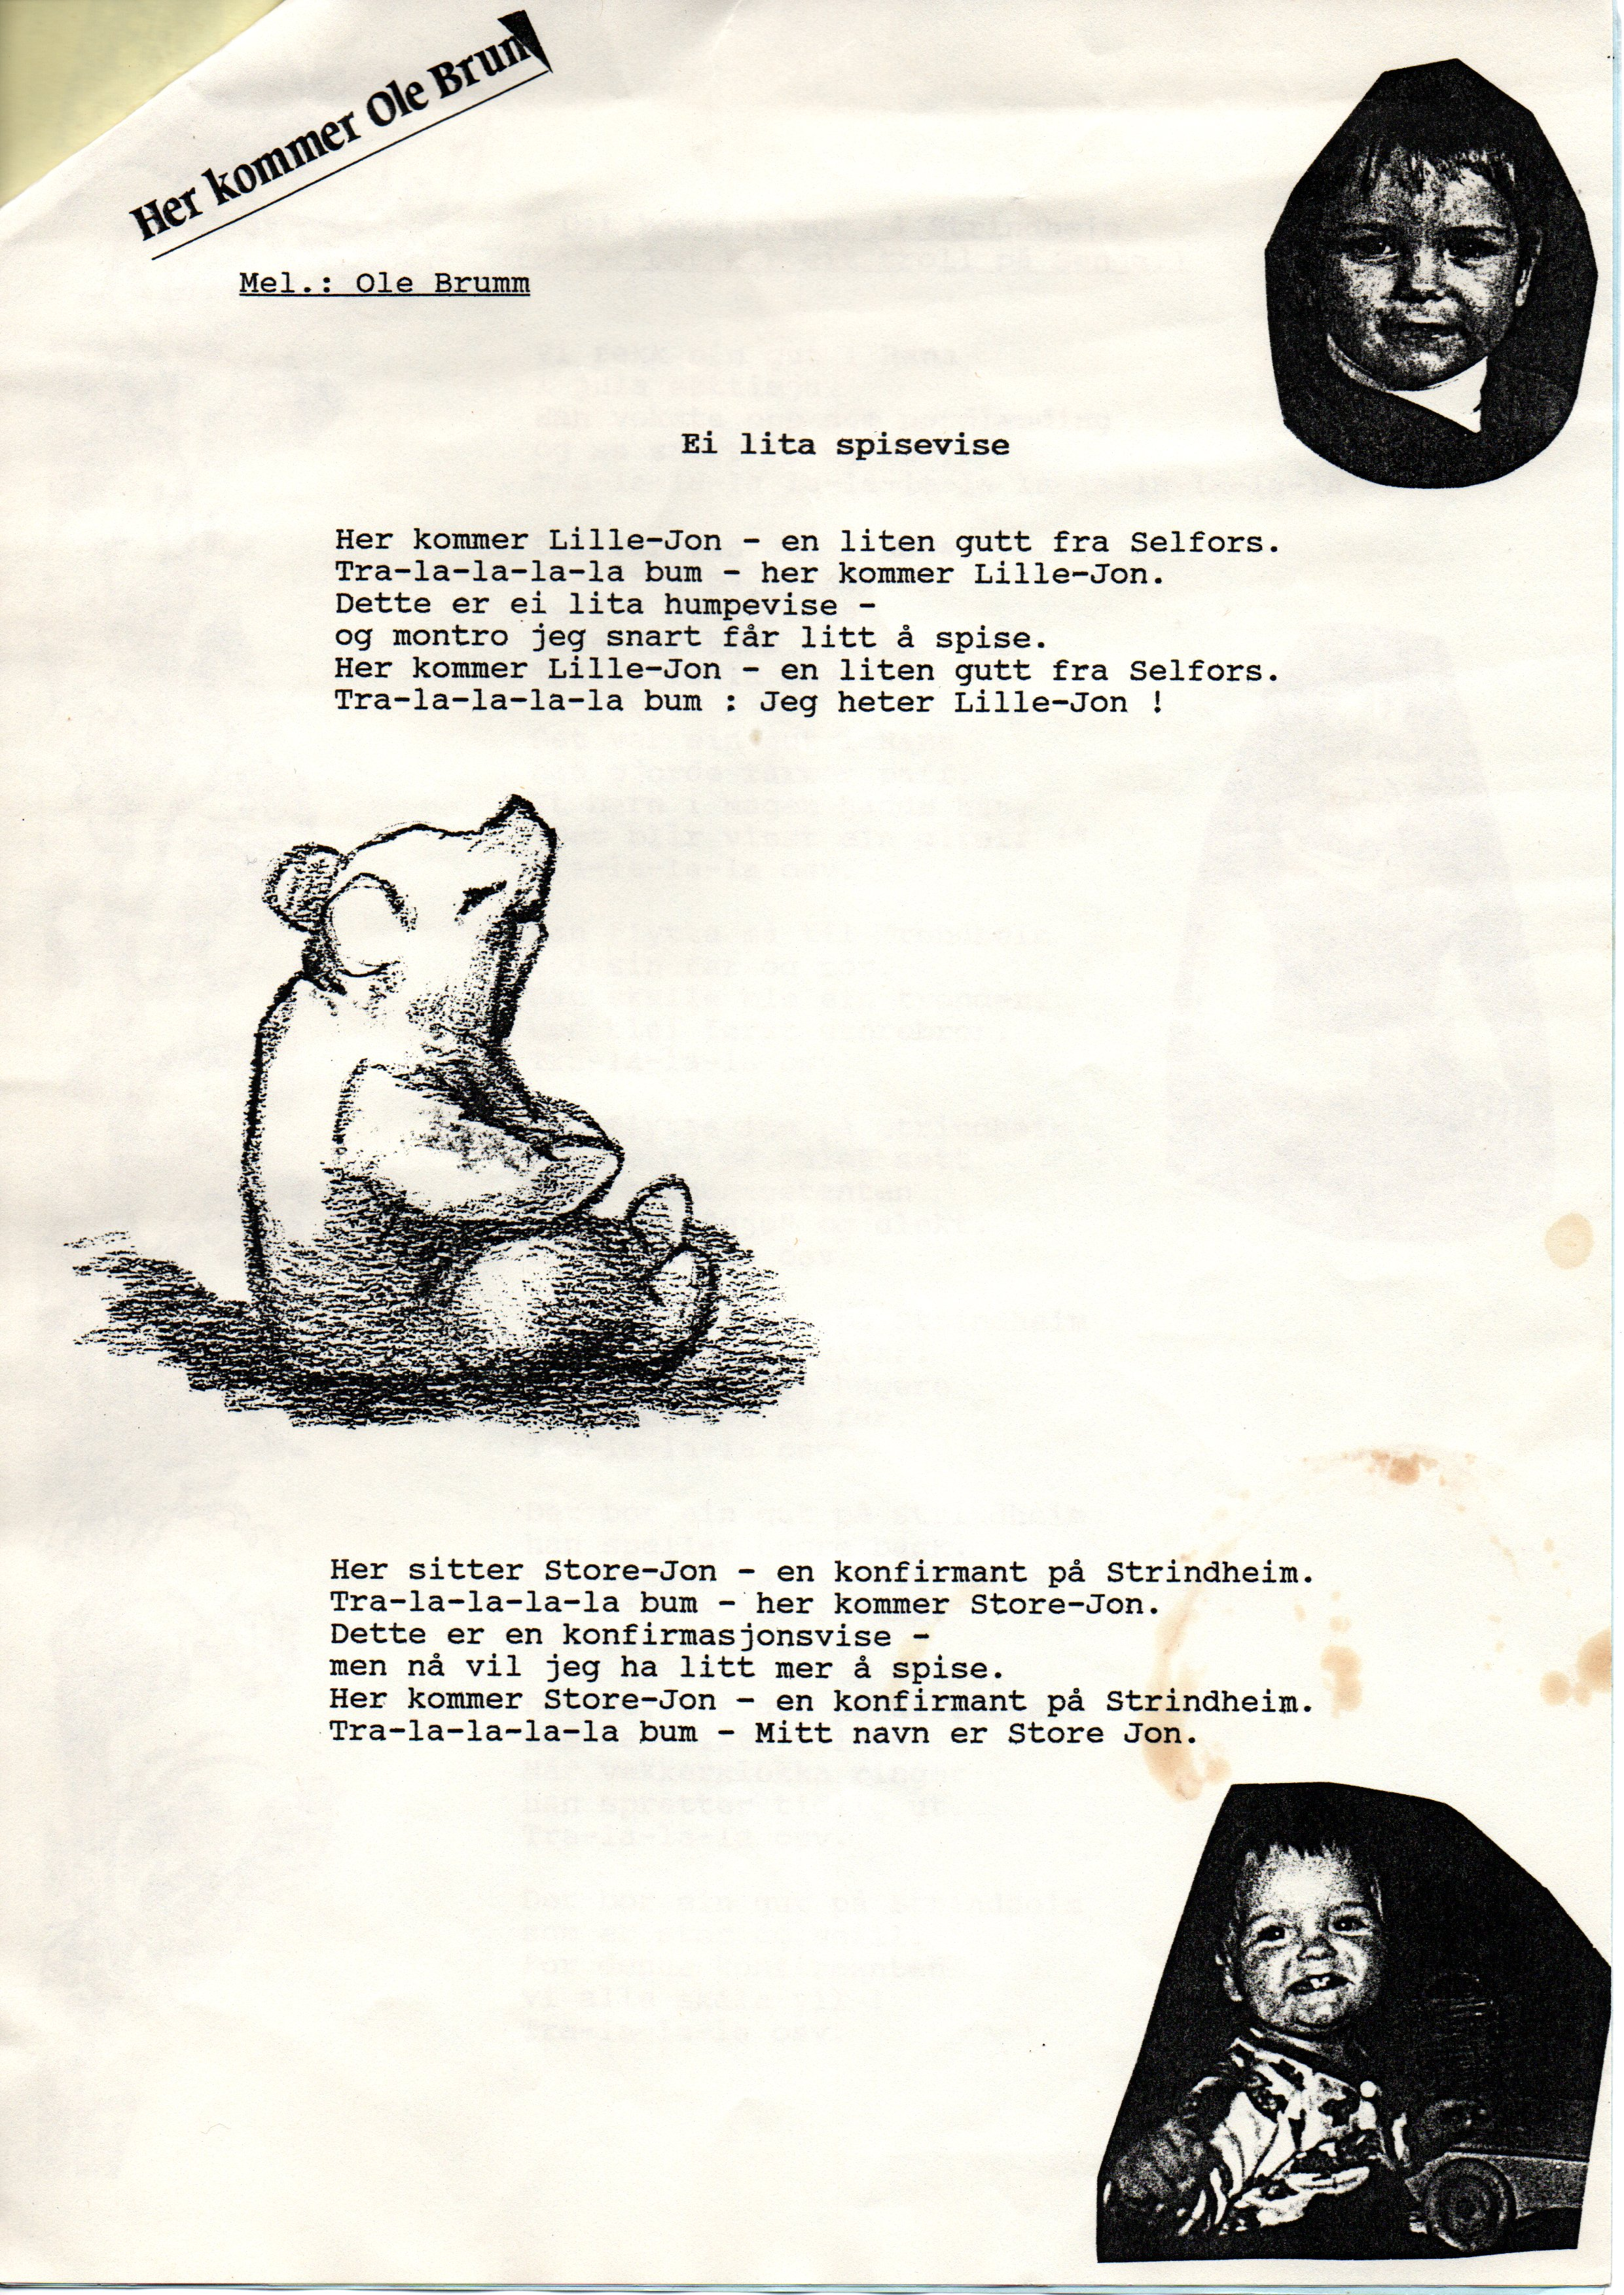
\includegraphics[width=0.97\textwidth]{illustrasjoner/jon2.jpg}
   \label{Jon2}
\end{figure}
\begin{figure}[H]
    \centering
    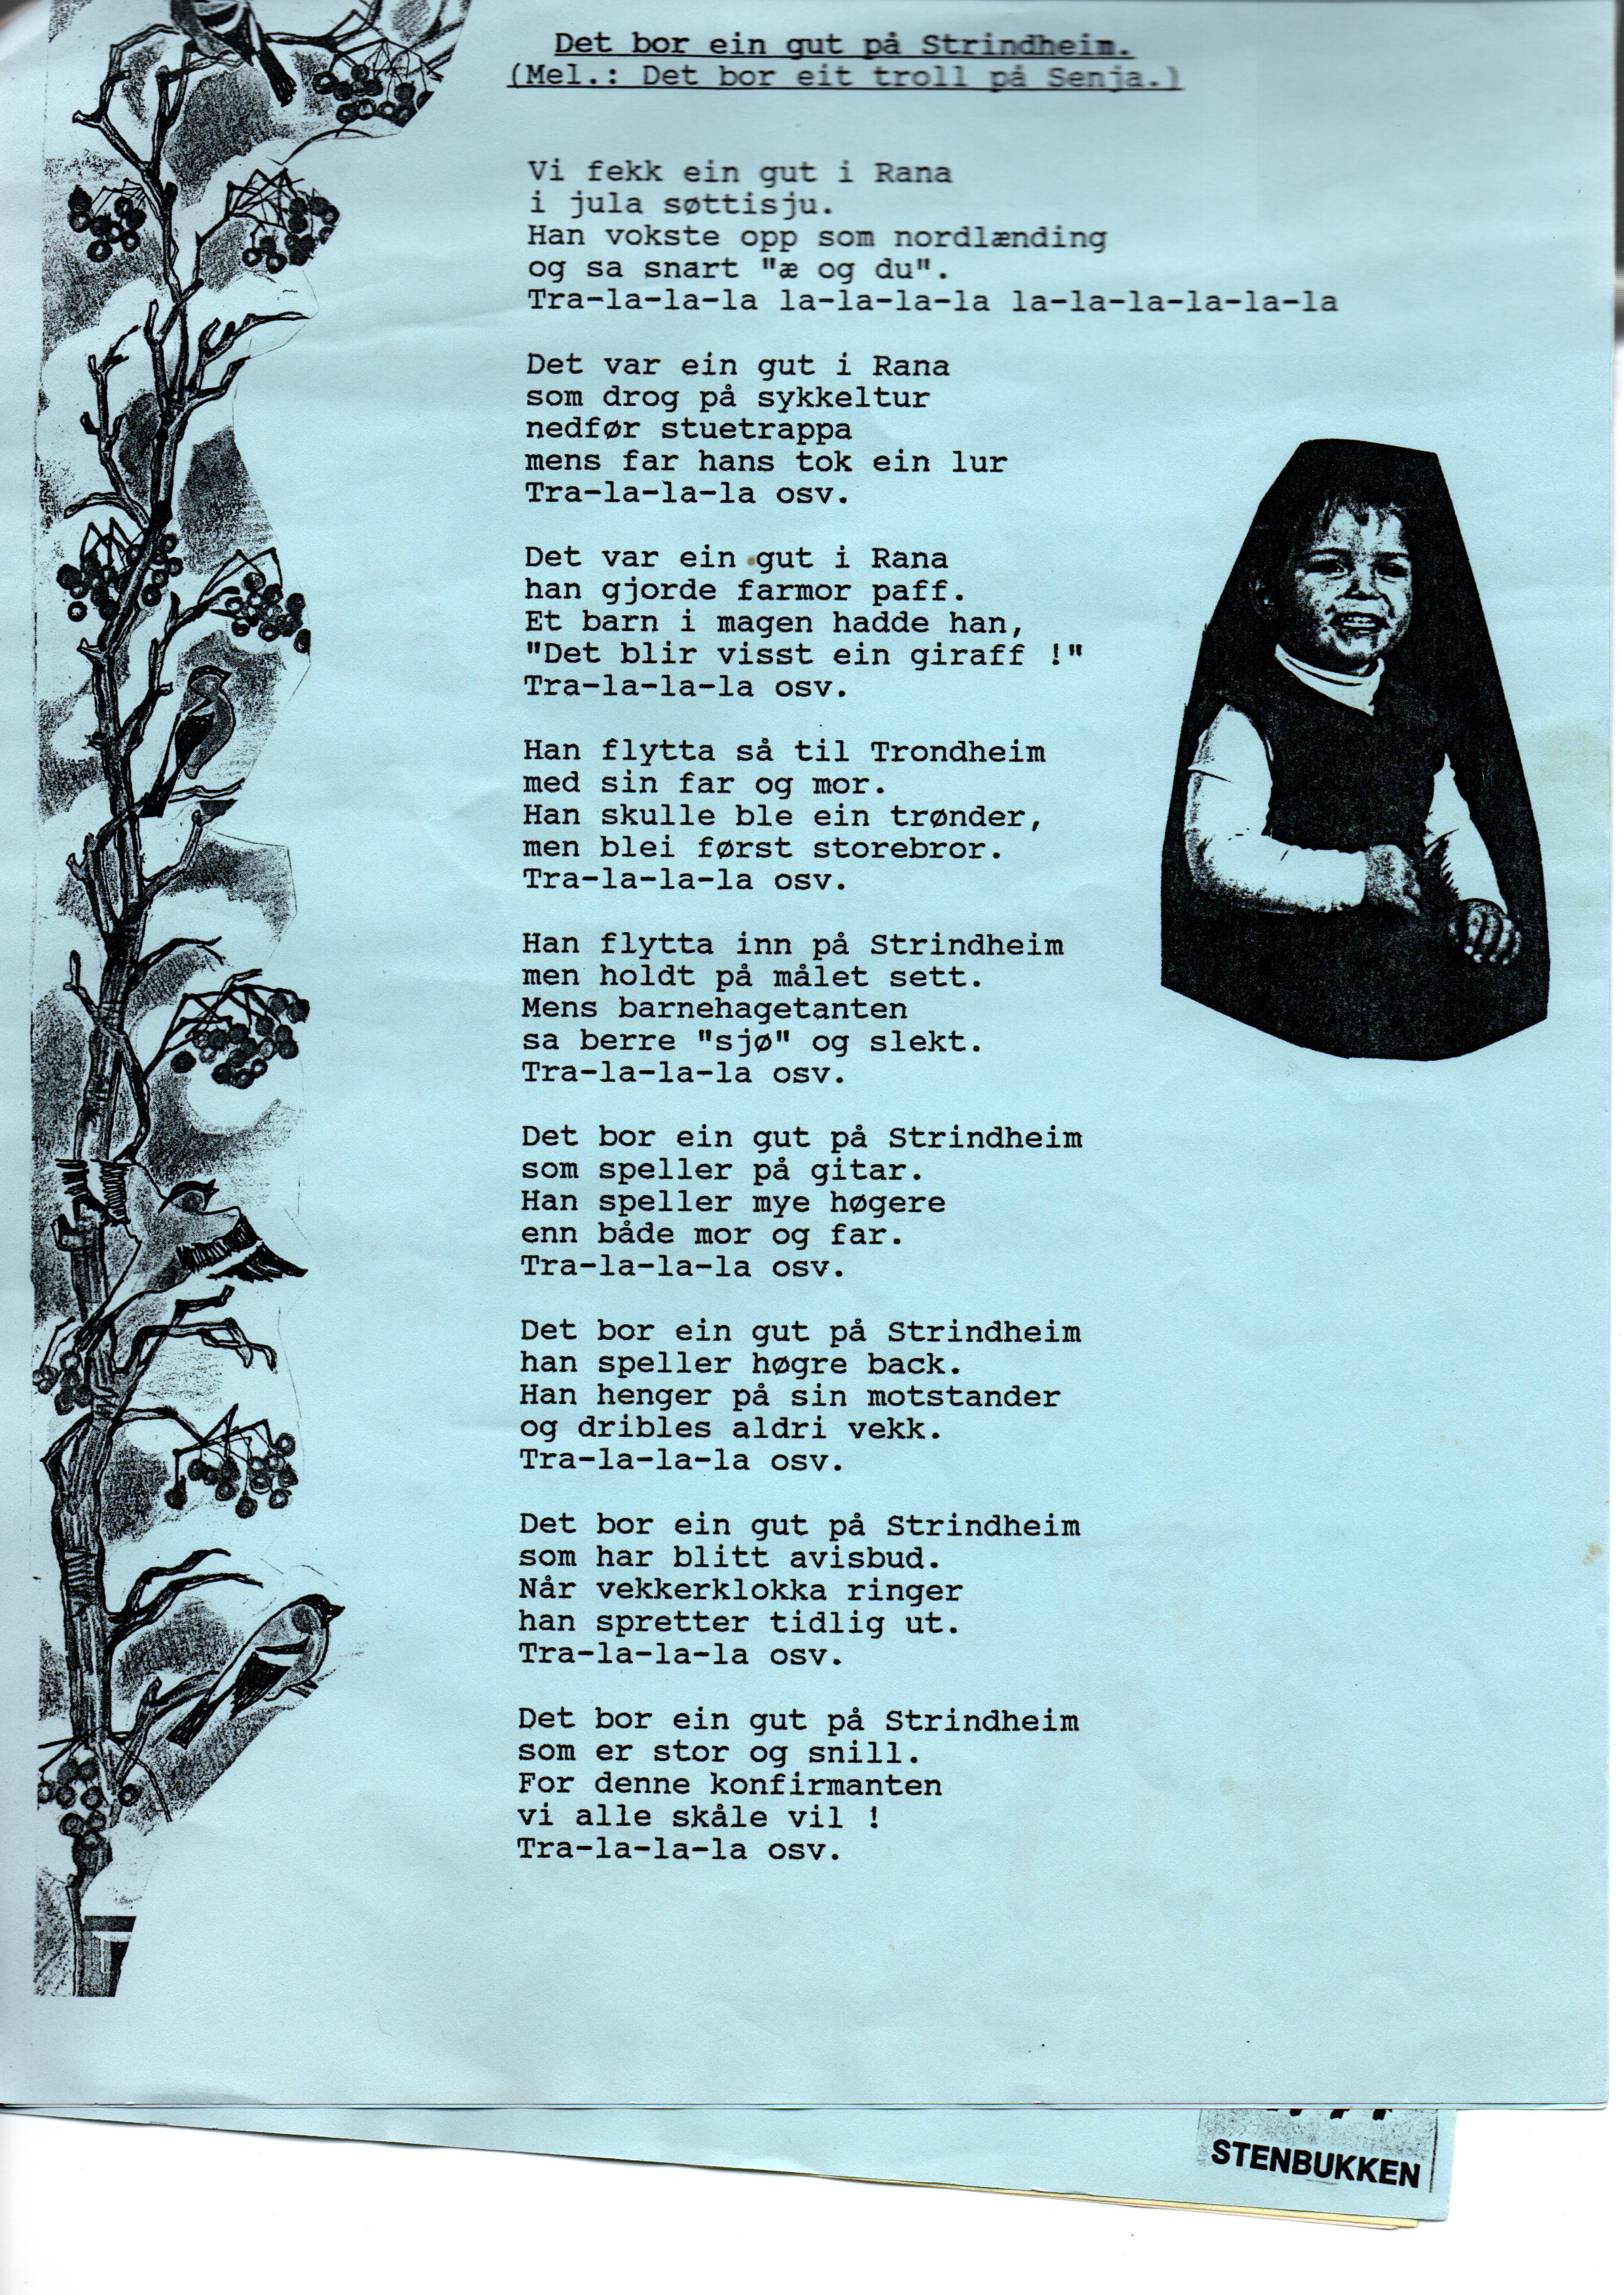
\includegraphics[width=0.97\textwidth]{illustrasjoner/jon3.jpg}
   \label{Jon3}
\end{figure}
\begin{figure}[H]
    \centering
    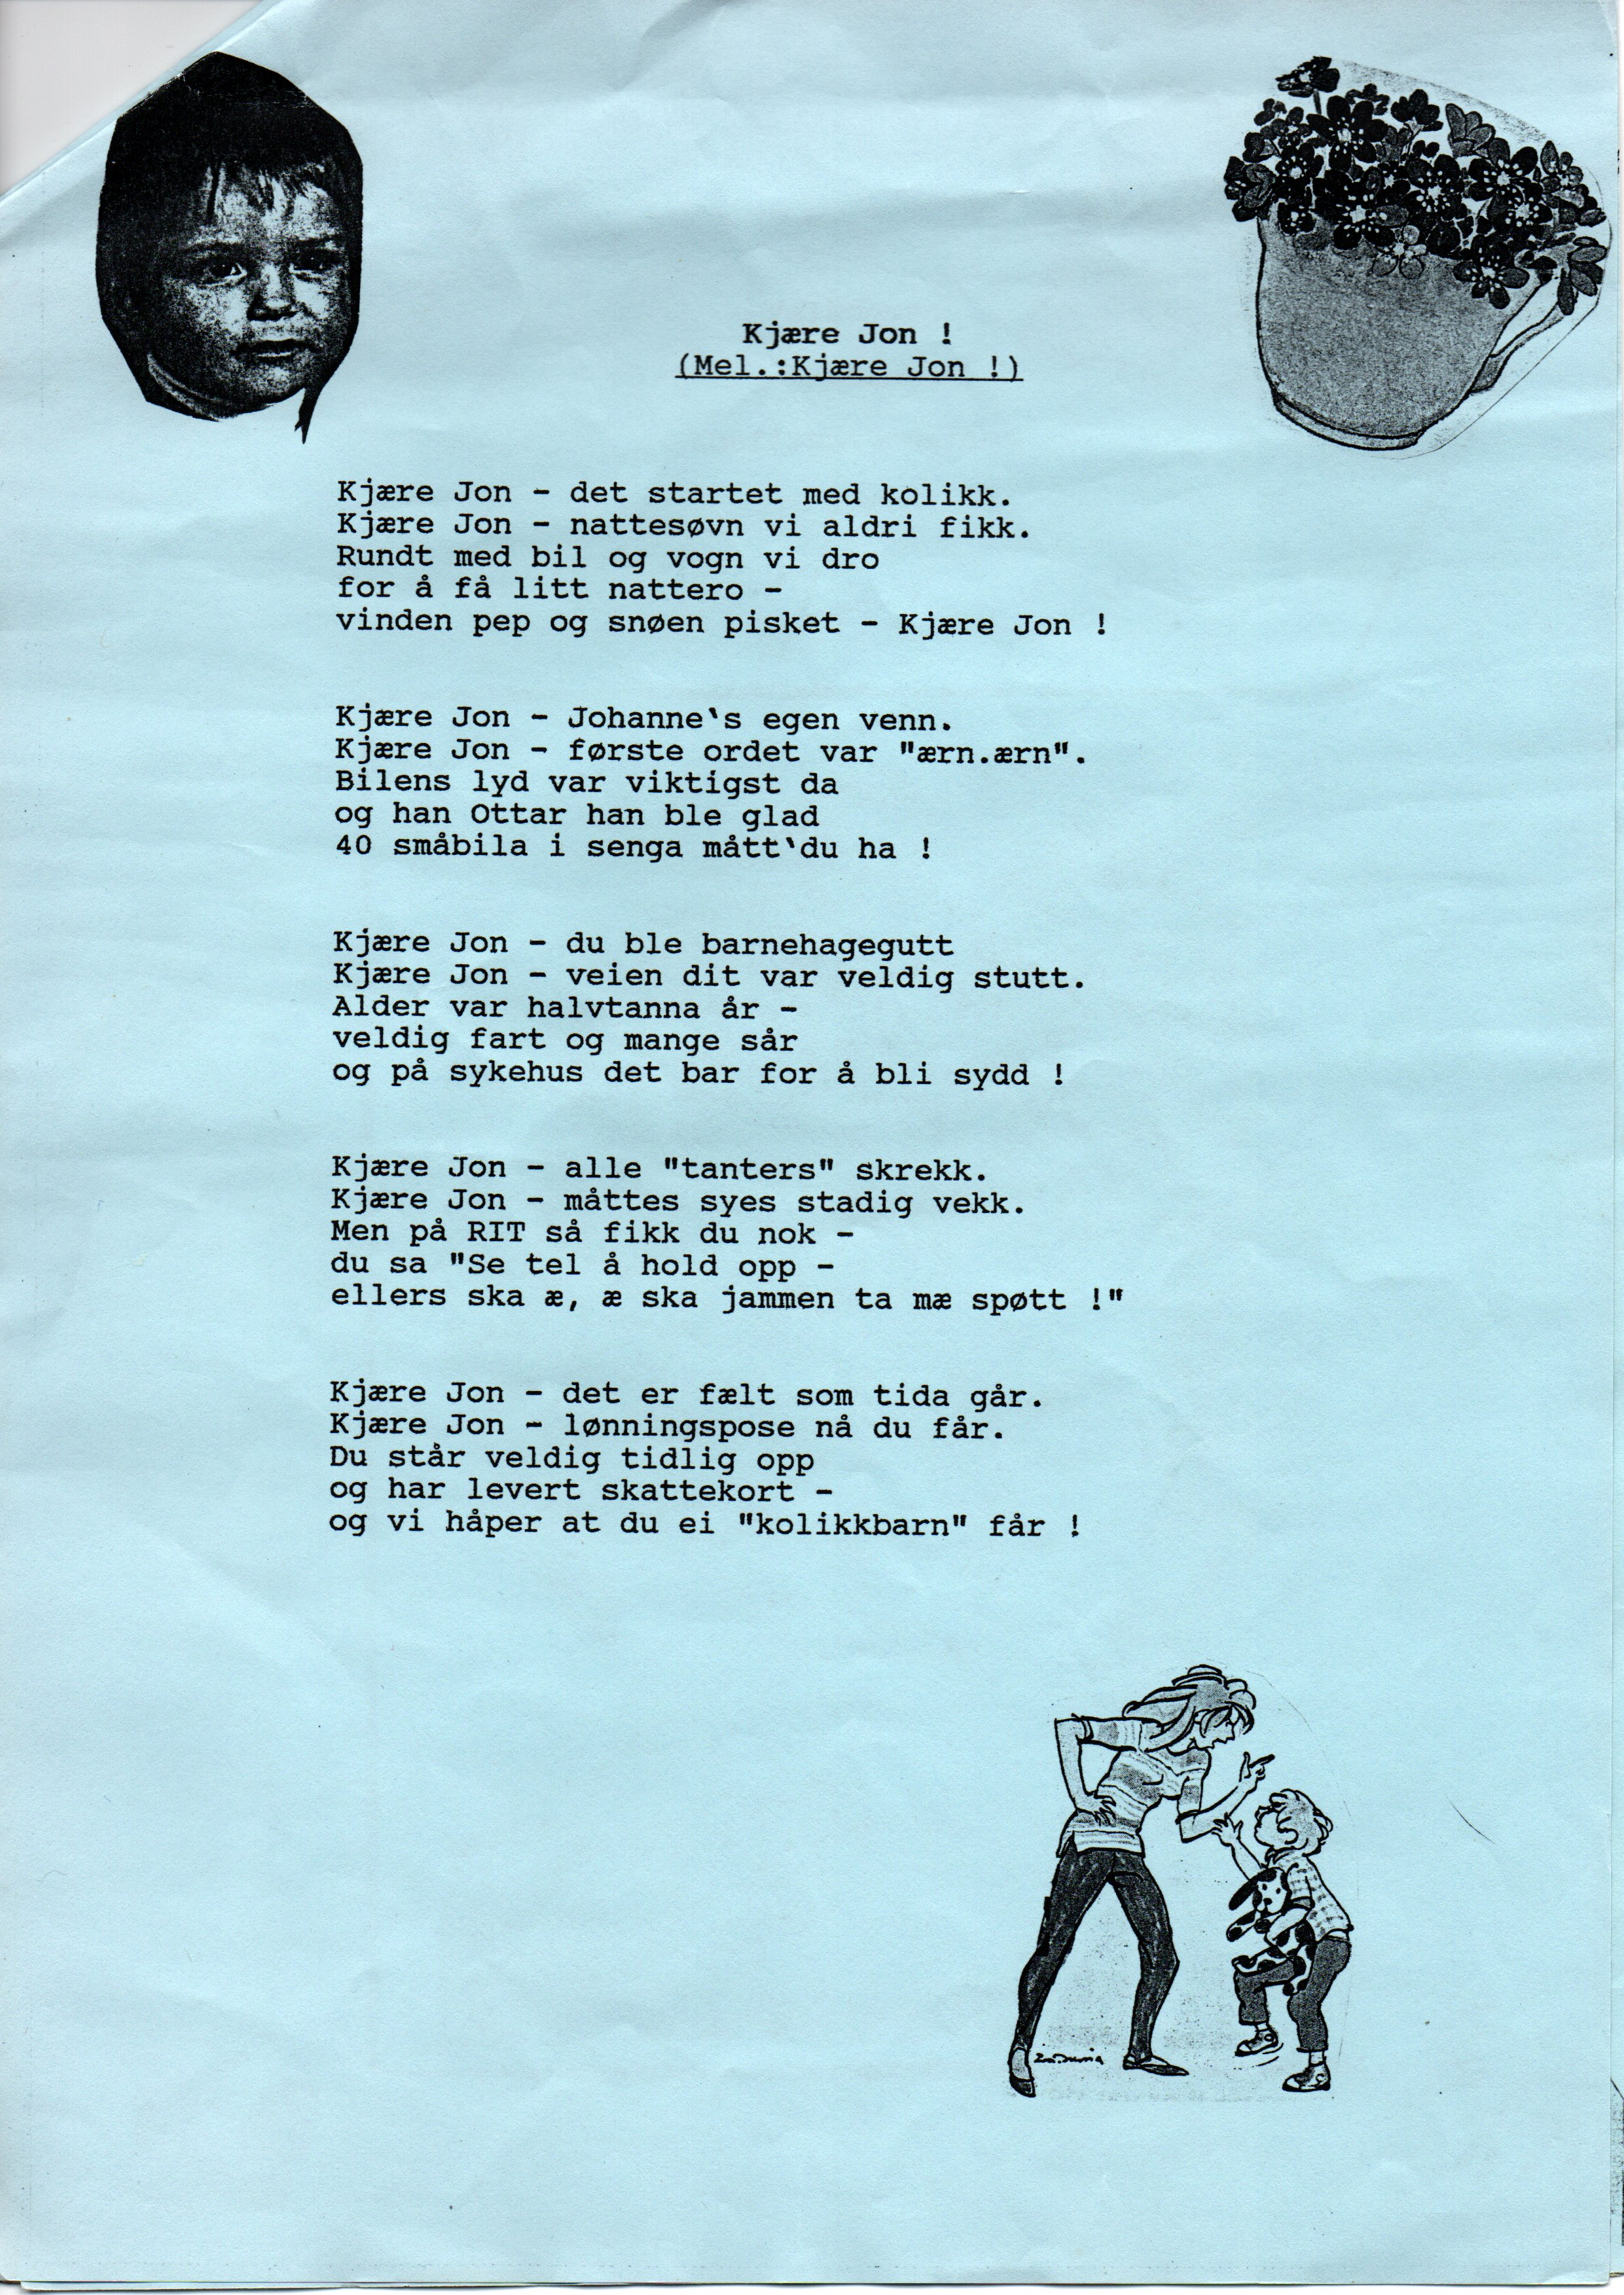
\includegraphics[width=0.97\textwidth]{illustrasjoner/jon4.jpg}
   \label{Jon4}
\end{figure}
\begin{figure}[H]
    \centering
    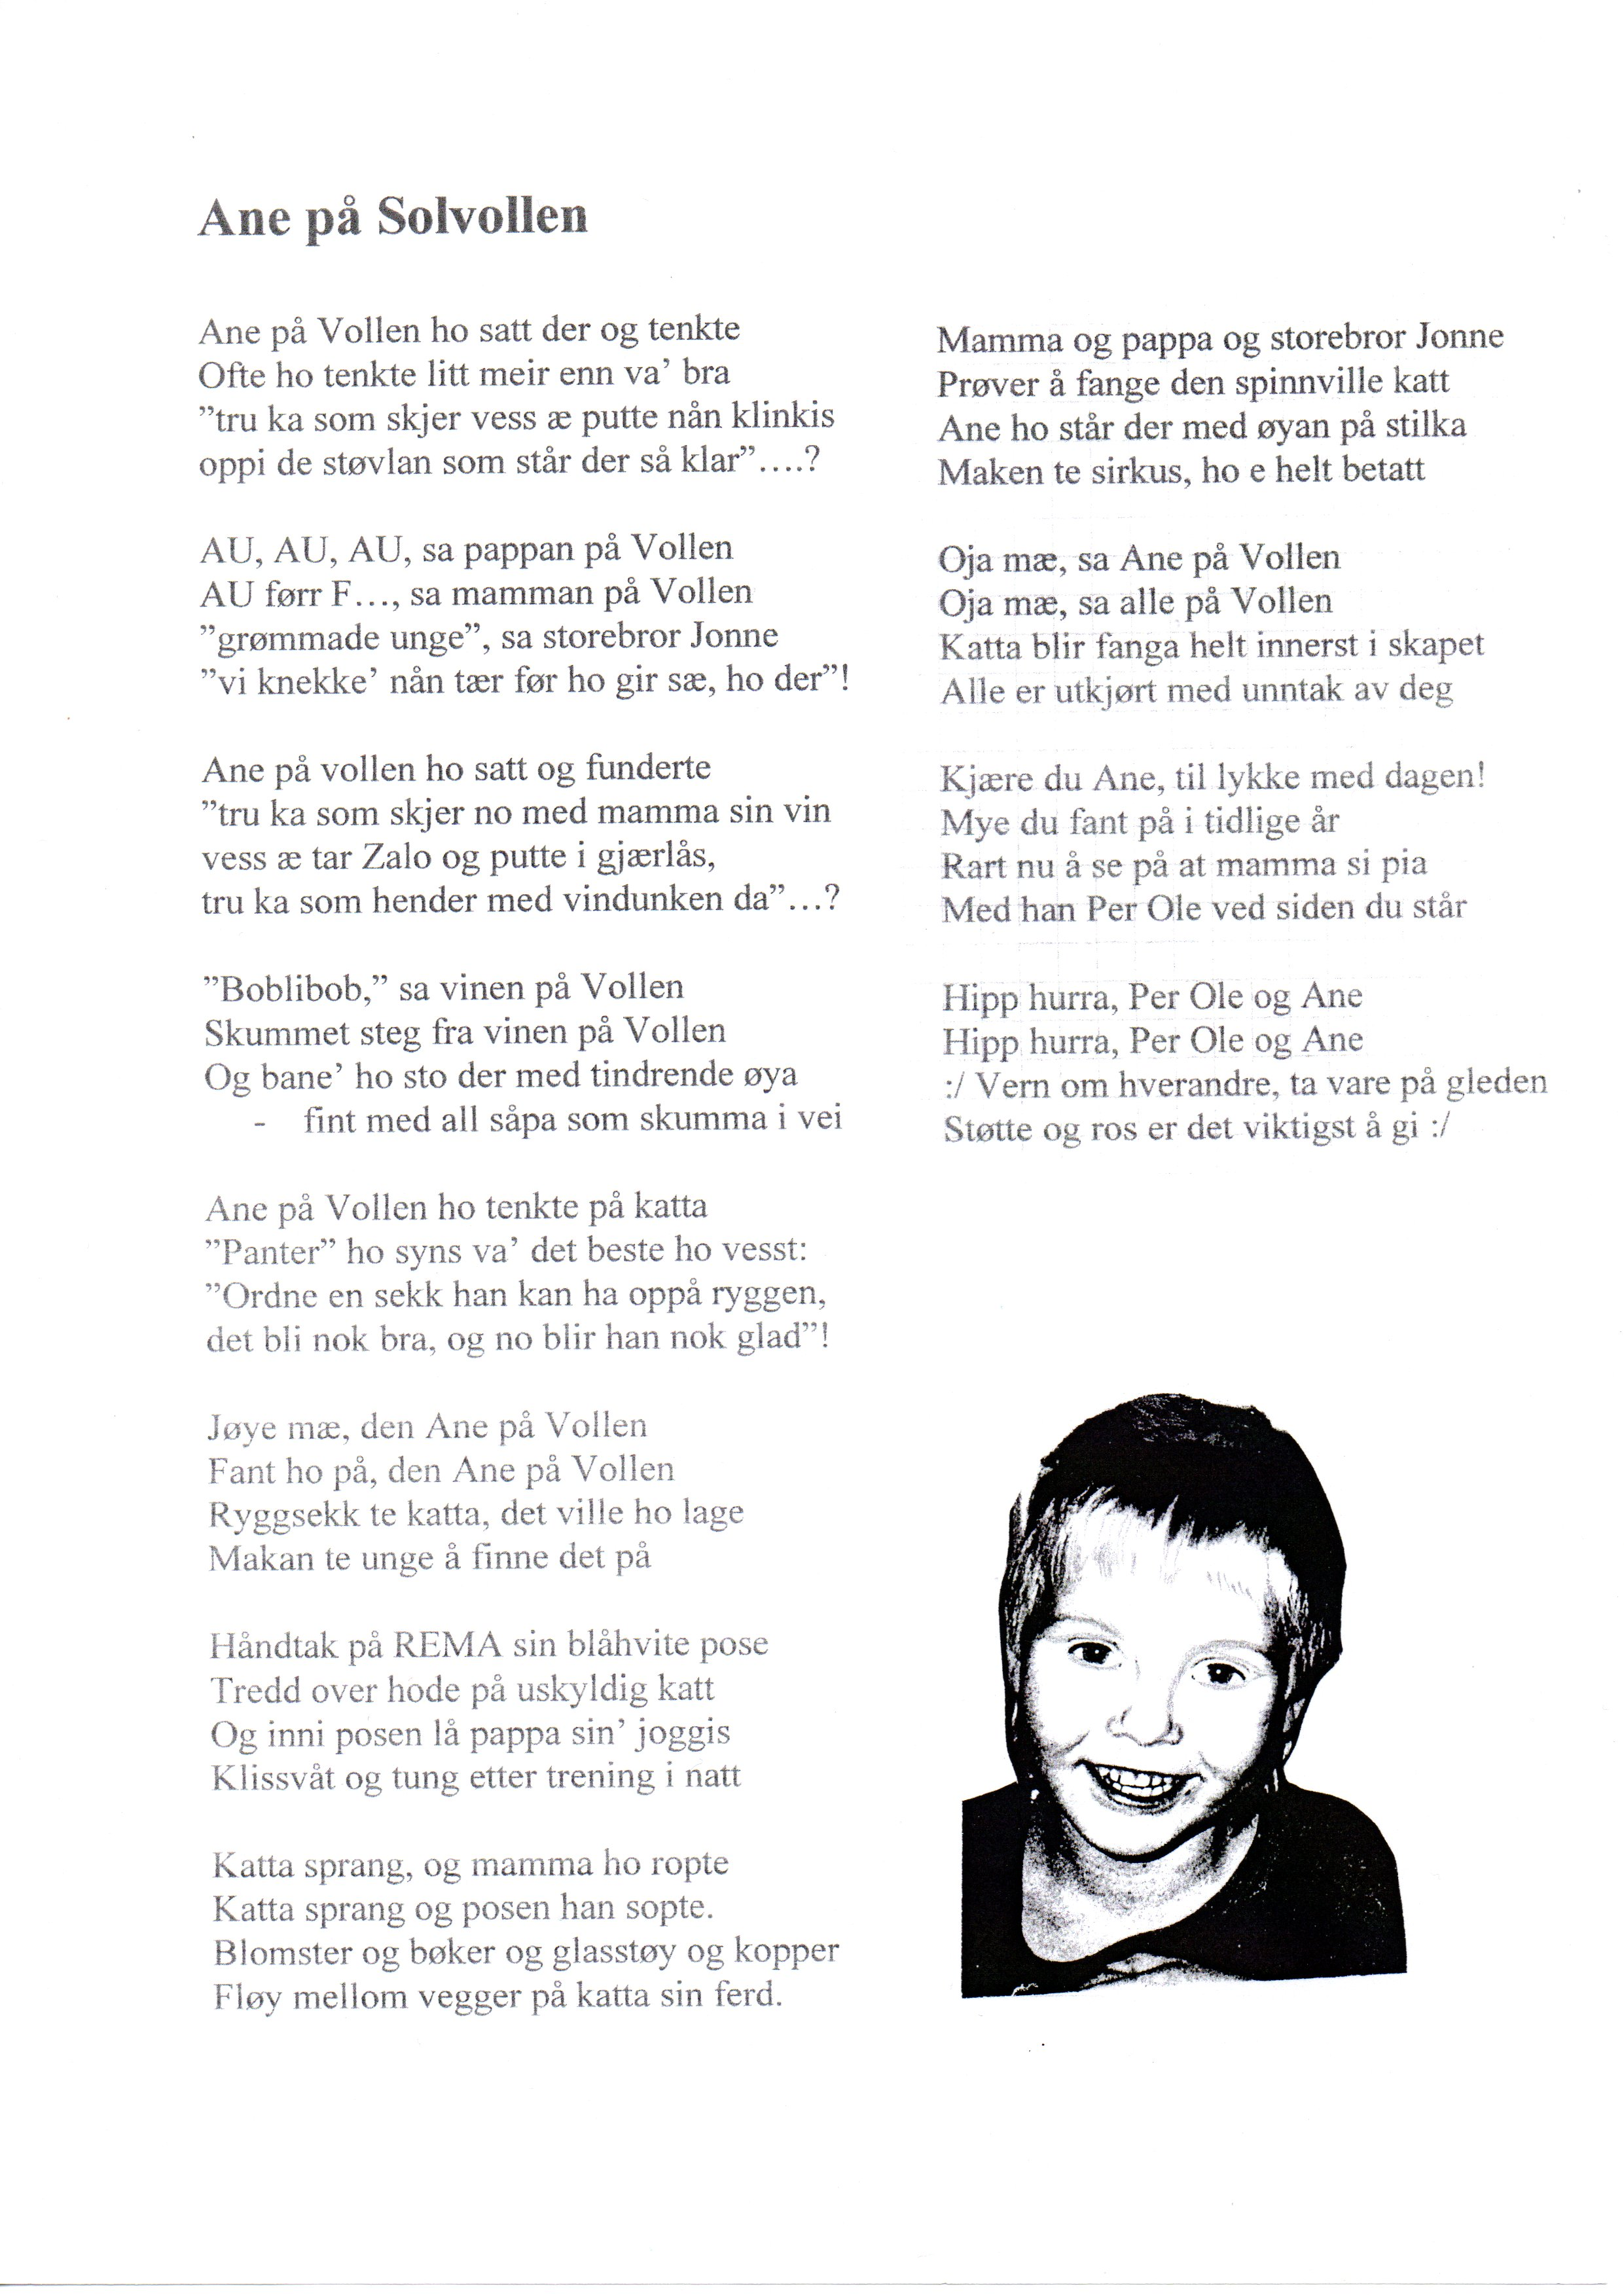
\includegraphics[width=0.97\textwidth]{illustrasjoner/ane1.jpg}
   \label{Ane1}
\end{figure}
\begin{figure}[H]
    \centering
    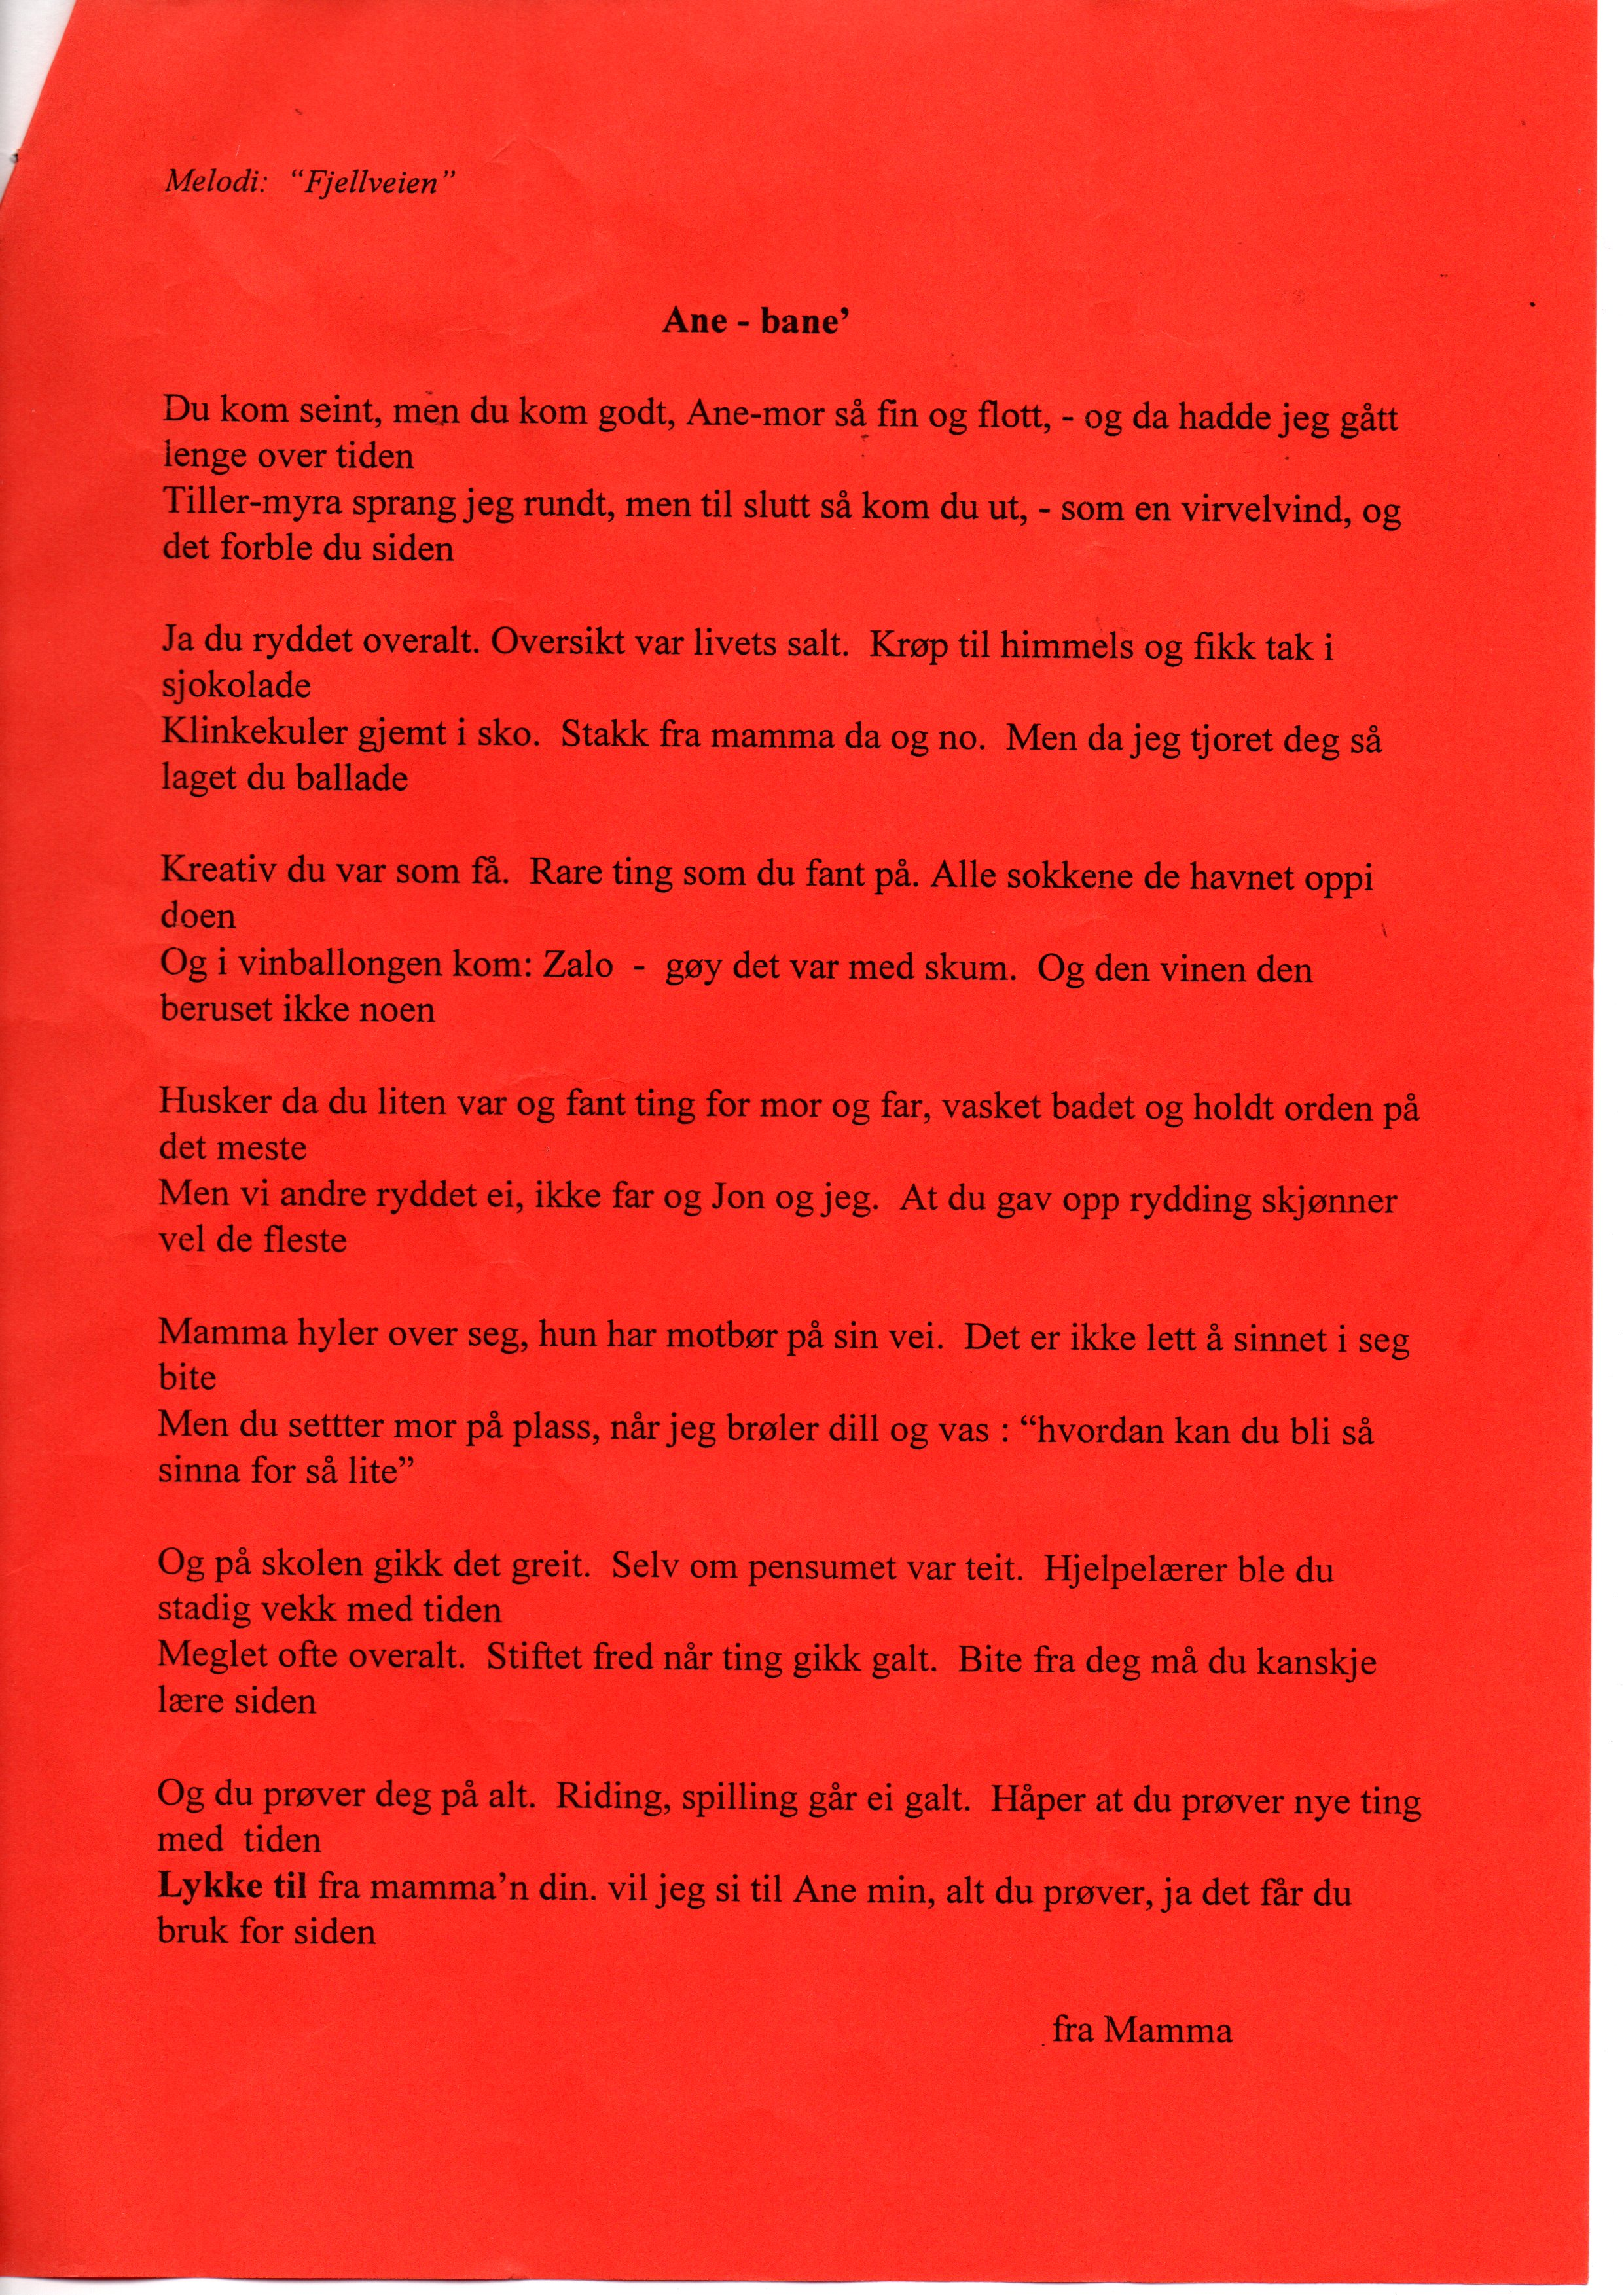
\includegraphics[width=0.97\textwidth]{illustrasjoner/ane2.jpg}
   \label{Ane2}
\end{figure}
\begin{figure}[H]
    \centering
    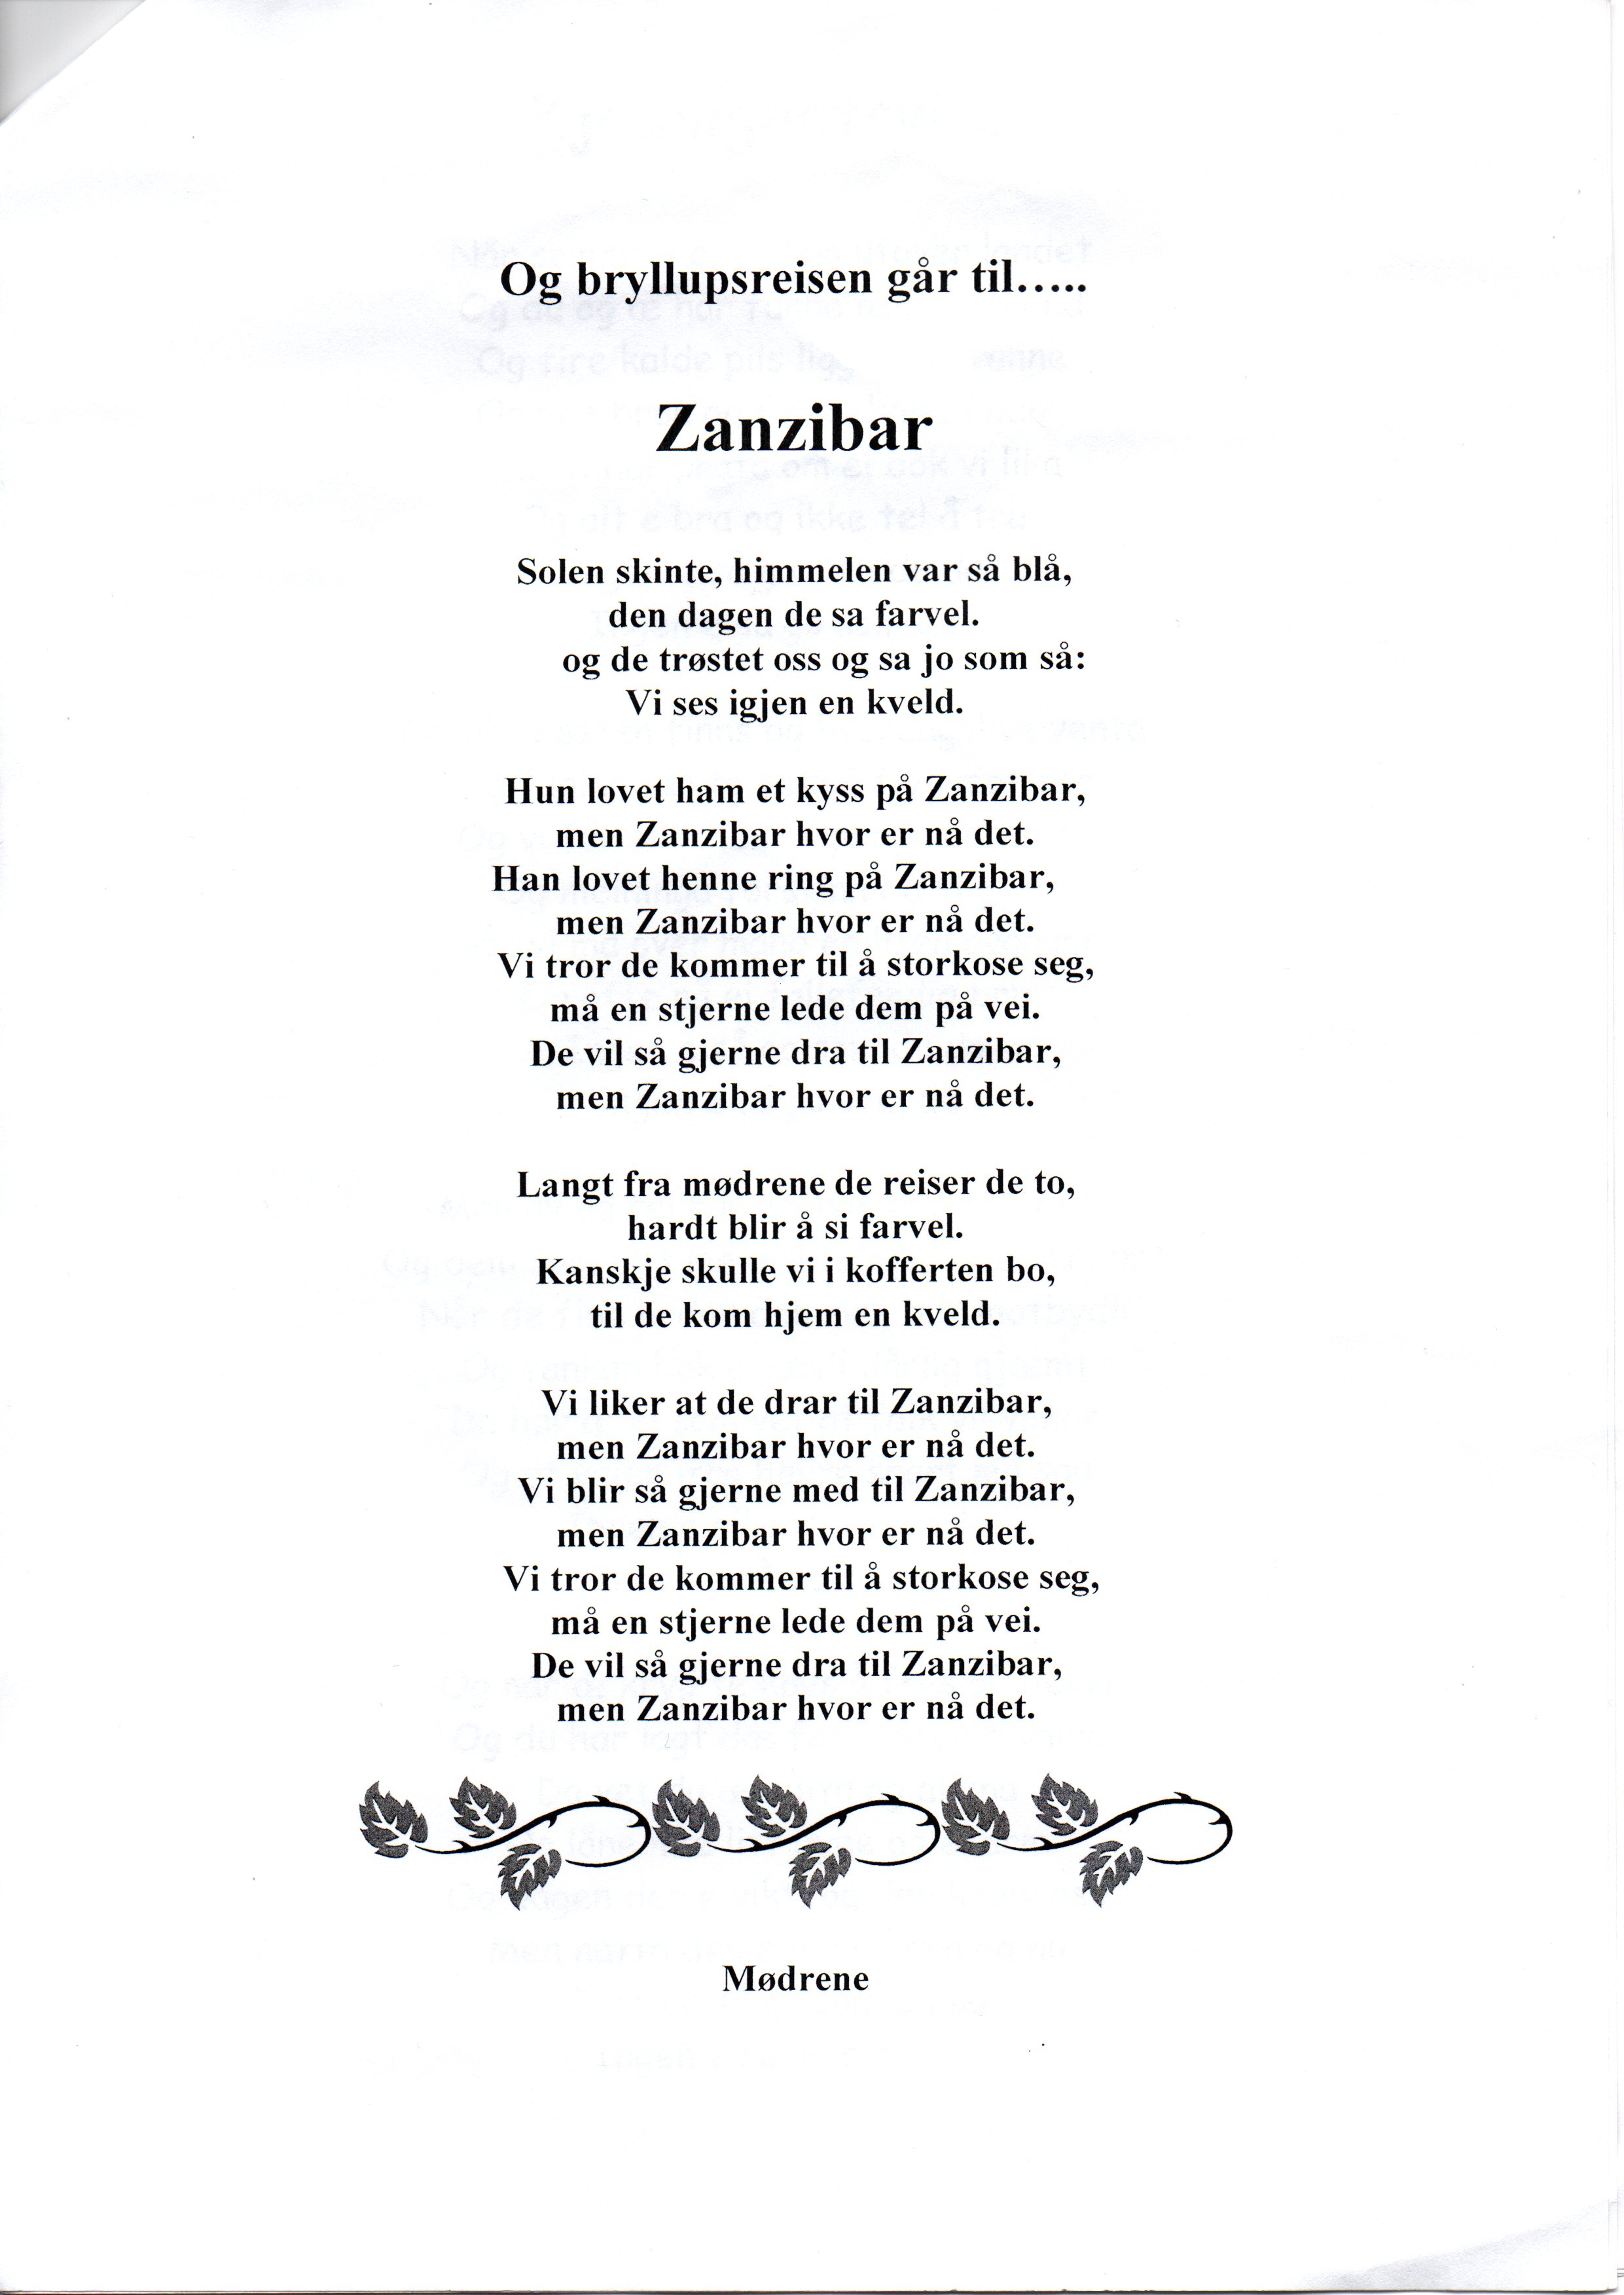
\includegraphics[width=0.97\textwidth]{illustrasjoner/Zanzibar.jpg}
   \label{Zanzibar}
\end{figure}


\chapter{Eventyrene til romfarer Dalsnes}
%\section{}
Det var en gang en veldig snill mormor som heter Lisbeth. Hun hadde oppdaget en helt ny planet.\\ Hun skulle egentlig på Pluto, men hun fikk noen problemer med motoren i romskipet. Så hun styrtet, men hun var magisk så hun overlevde.\\ Hun så seg rundt og oppdaget at alt var av godteri.\\
\begin{figure}[H]
    \centering
    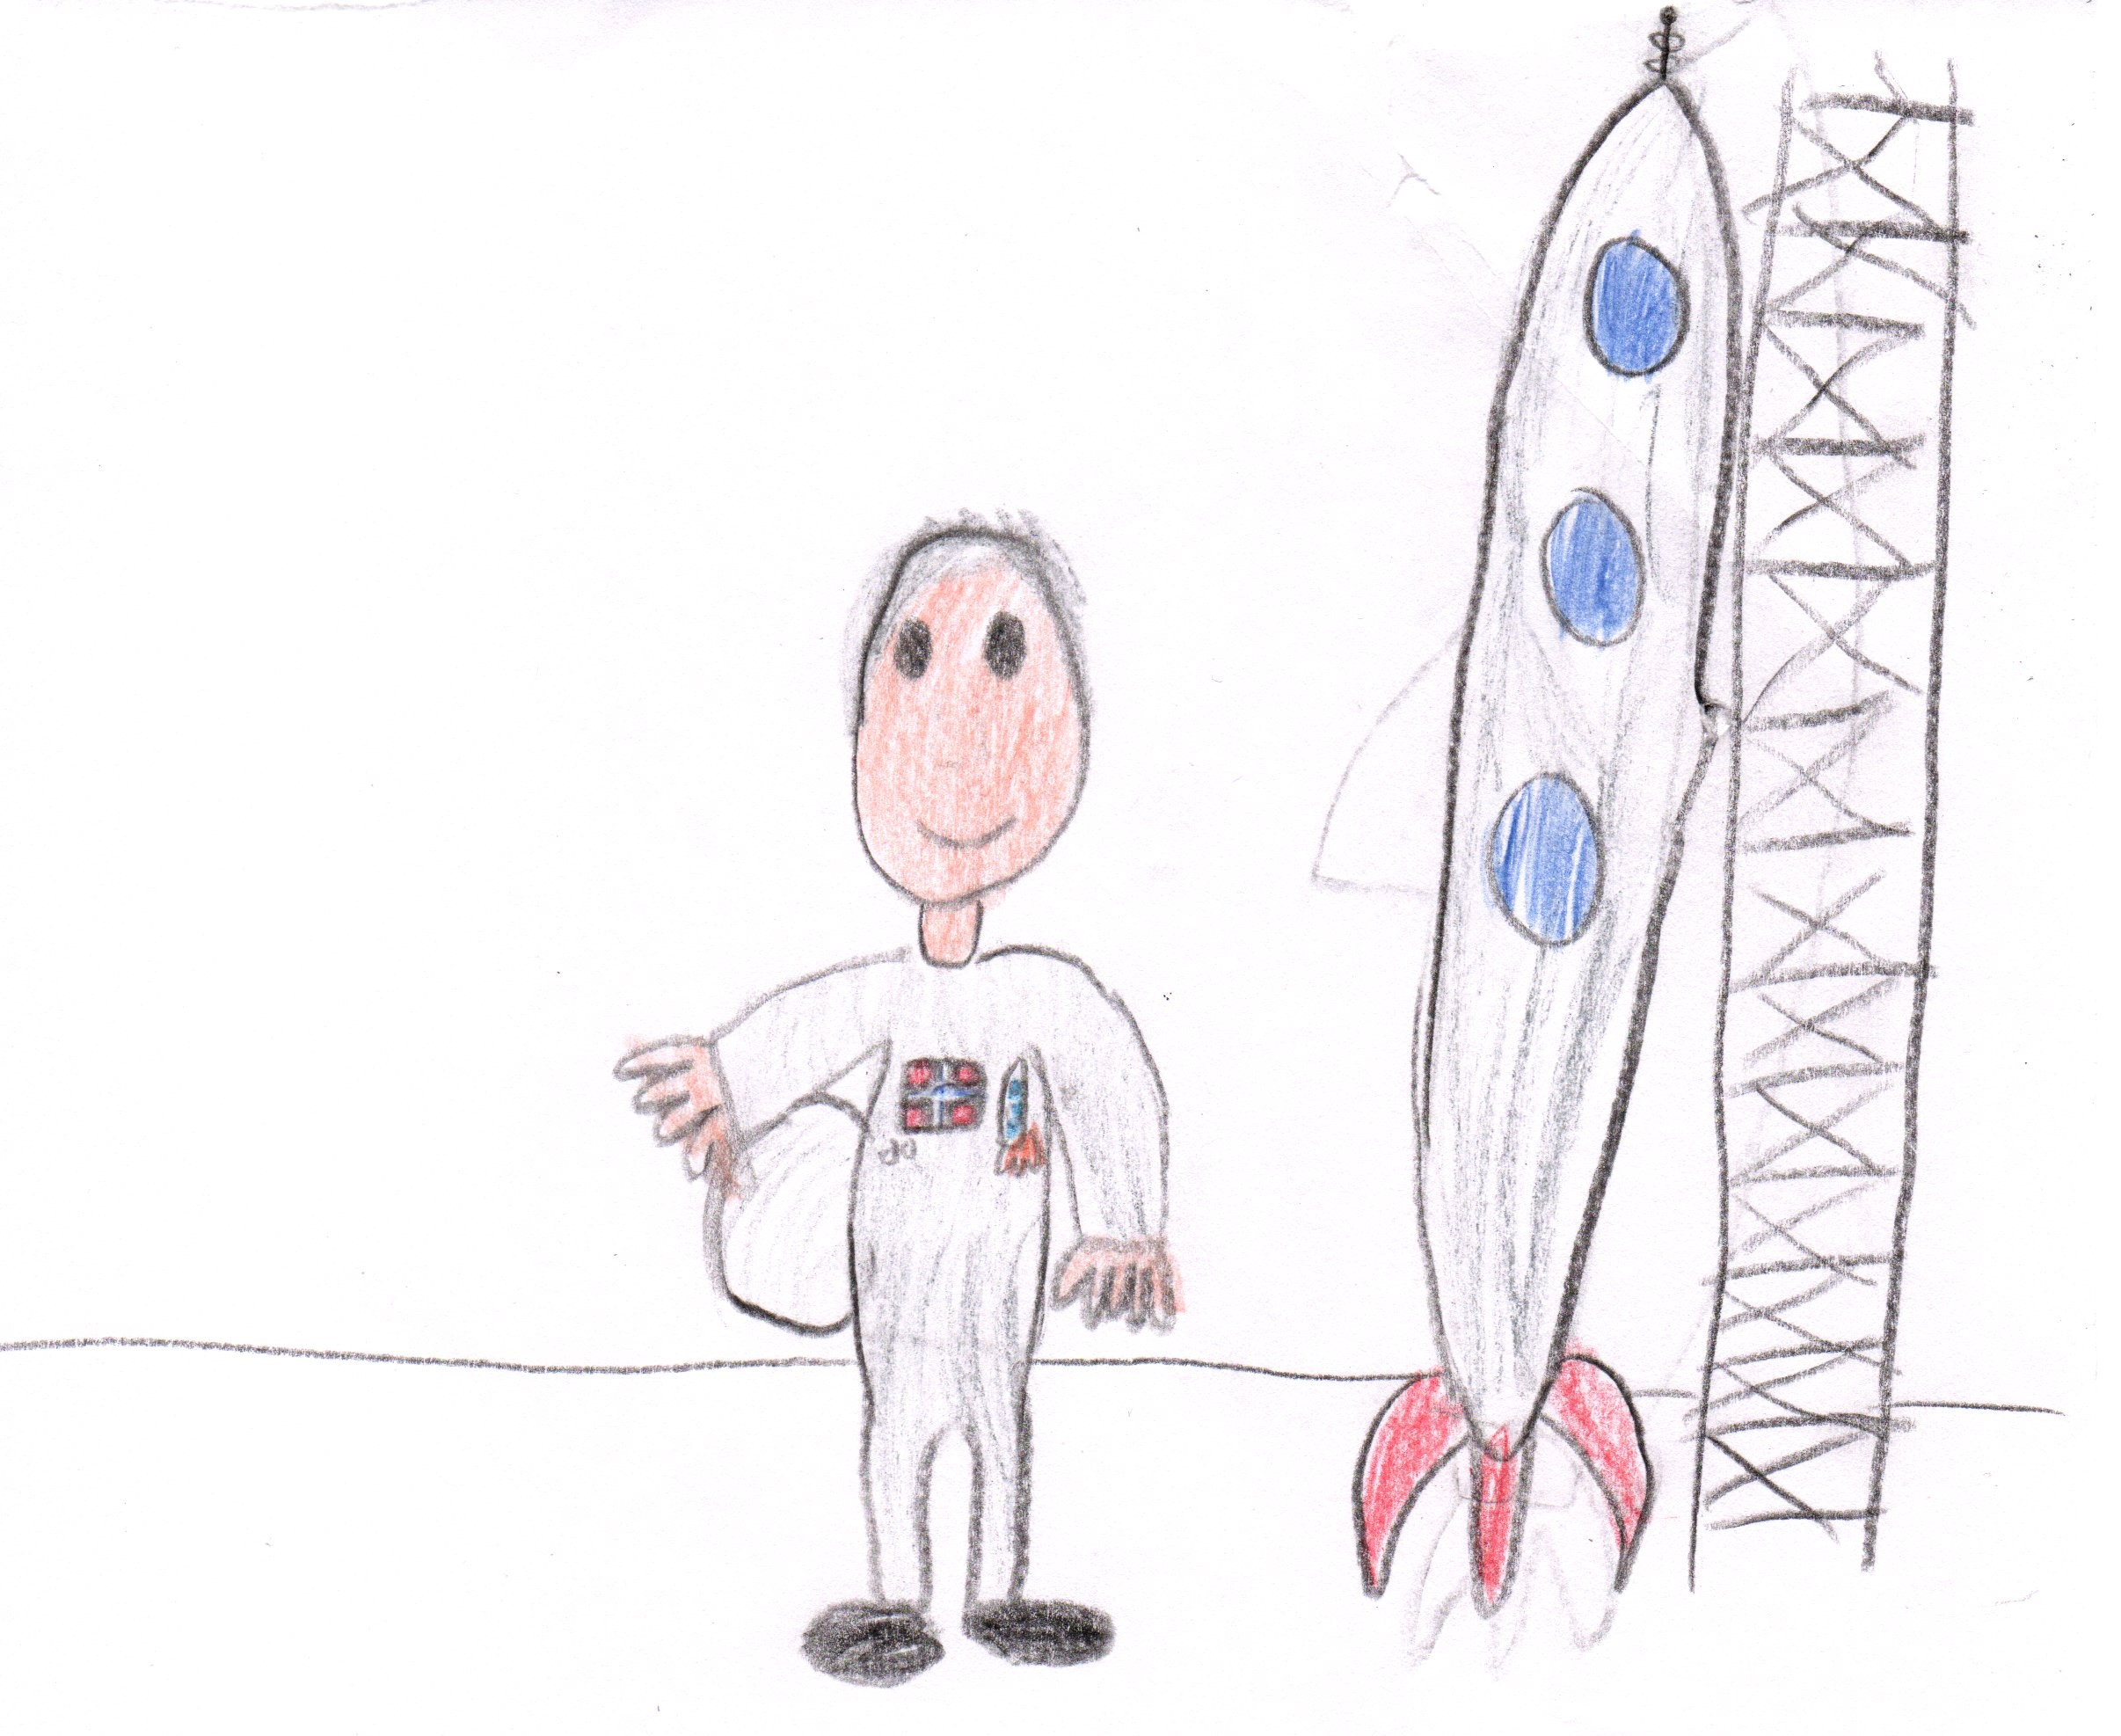
\includegraphics[width=0.8\textwidth]{illustrasjoner/Lisbethromfarer.jpg}
   \label{romfarer}
   \caption{Romfarer Dalsnes av Oline}
\end{figure}

Hun måtte finne på et navn til planeten. Hun fant på et morsomt navn. \textit{Knask og godt} var navnet  til planeten.\hfill \newline\\ 
Skyene var av sukkerspinn. Noen sukkerspinnskyer var rosa, noen var grønne og noen var blåe og de hadde strøssel. Stammen til trærene var av lakris og bladene var av sjokolade med grønn konditorfarge! Og den vakreste fossen av smeltet melkesjokolade rant rett ved siden av den ødelagte romskipet. Steinene var av marshmallow og husene var av pepperkaker.\\
\hfill \newline
Hun prøvde og ringe til folket i byen hennes, men det var ikke dekning på planeten. Så hun måtte bli der. Menneskene var ikke menesker, men seigmenn og de hadde ikke hunder og katter til kjæledyr men de hadde gummibjørner som kjæledyr.\\
\hfill \newline 
Hun lagde seg et hus av pepperkake og flyttet inn i byen. Hun fikk noen venner i byen fordi selv om  det bare var seigmenner i byen kunne de snakke.\\
\hfill \newline
Hun var så snill at hun fikk snill-superkrefter! Det kom ofte meteoritter til byen men hun stoppet dem med snill-superkreftene sine. Hun kunne fly og hun ville oppdage flere matrealer fra andre planeter, men hun lovte og komme tilbake. \\
\hfill \newline
Hun oppdaget en planet av myke ting hun kalte den Kose-planeten og der var det allemulige ting som var helt myke. Og hun oppdaget en planet som hun kalte Ferie-planeten, der var det bare skole på torsdager. Der holt barna på med og lage fine ting i stede for og ha skole. Etter det dro hun til en ny planet hun kalte den Regnbue-planeten. Der var det kjempe mange regnbuer og de fleste var veldig store!
%%%%%%%%%%%%%%%%%%%%%%%%%%%%%%%%%%%%%%%%%%%%%%%%%%%%%%%
\section{Monsterplaneten}bb
\begin{figure}[H]
    \centering
    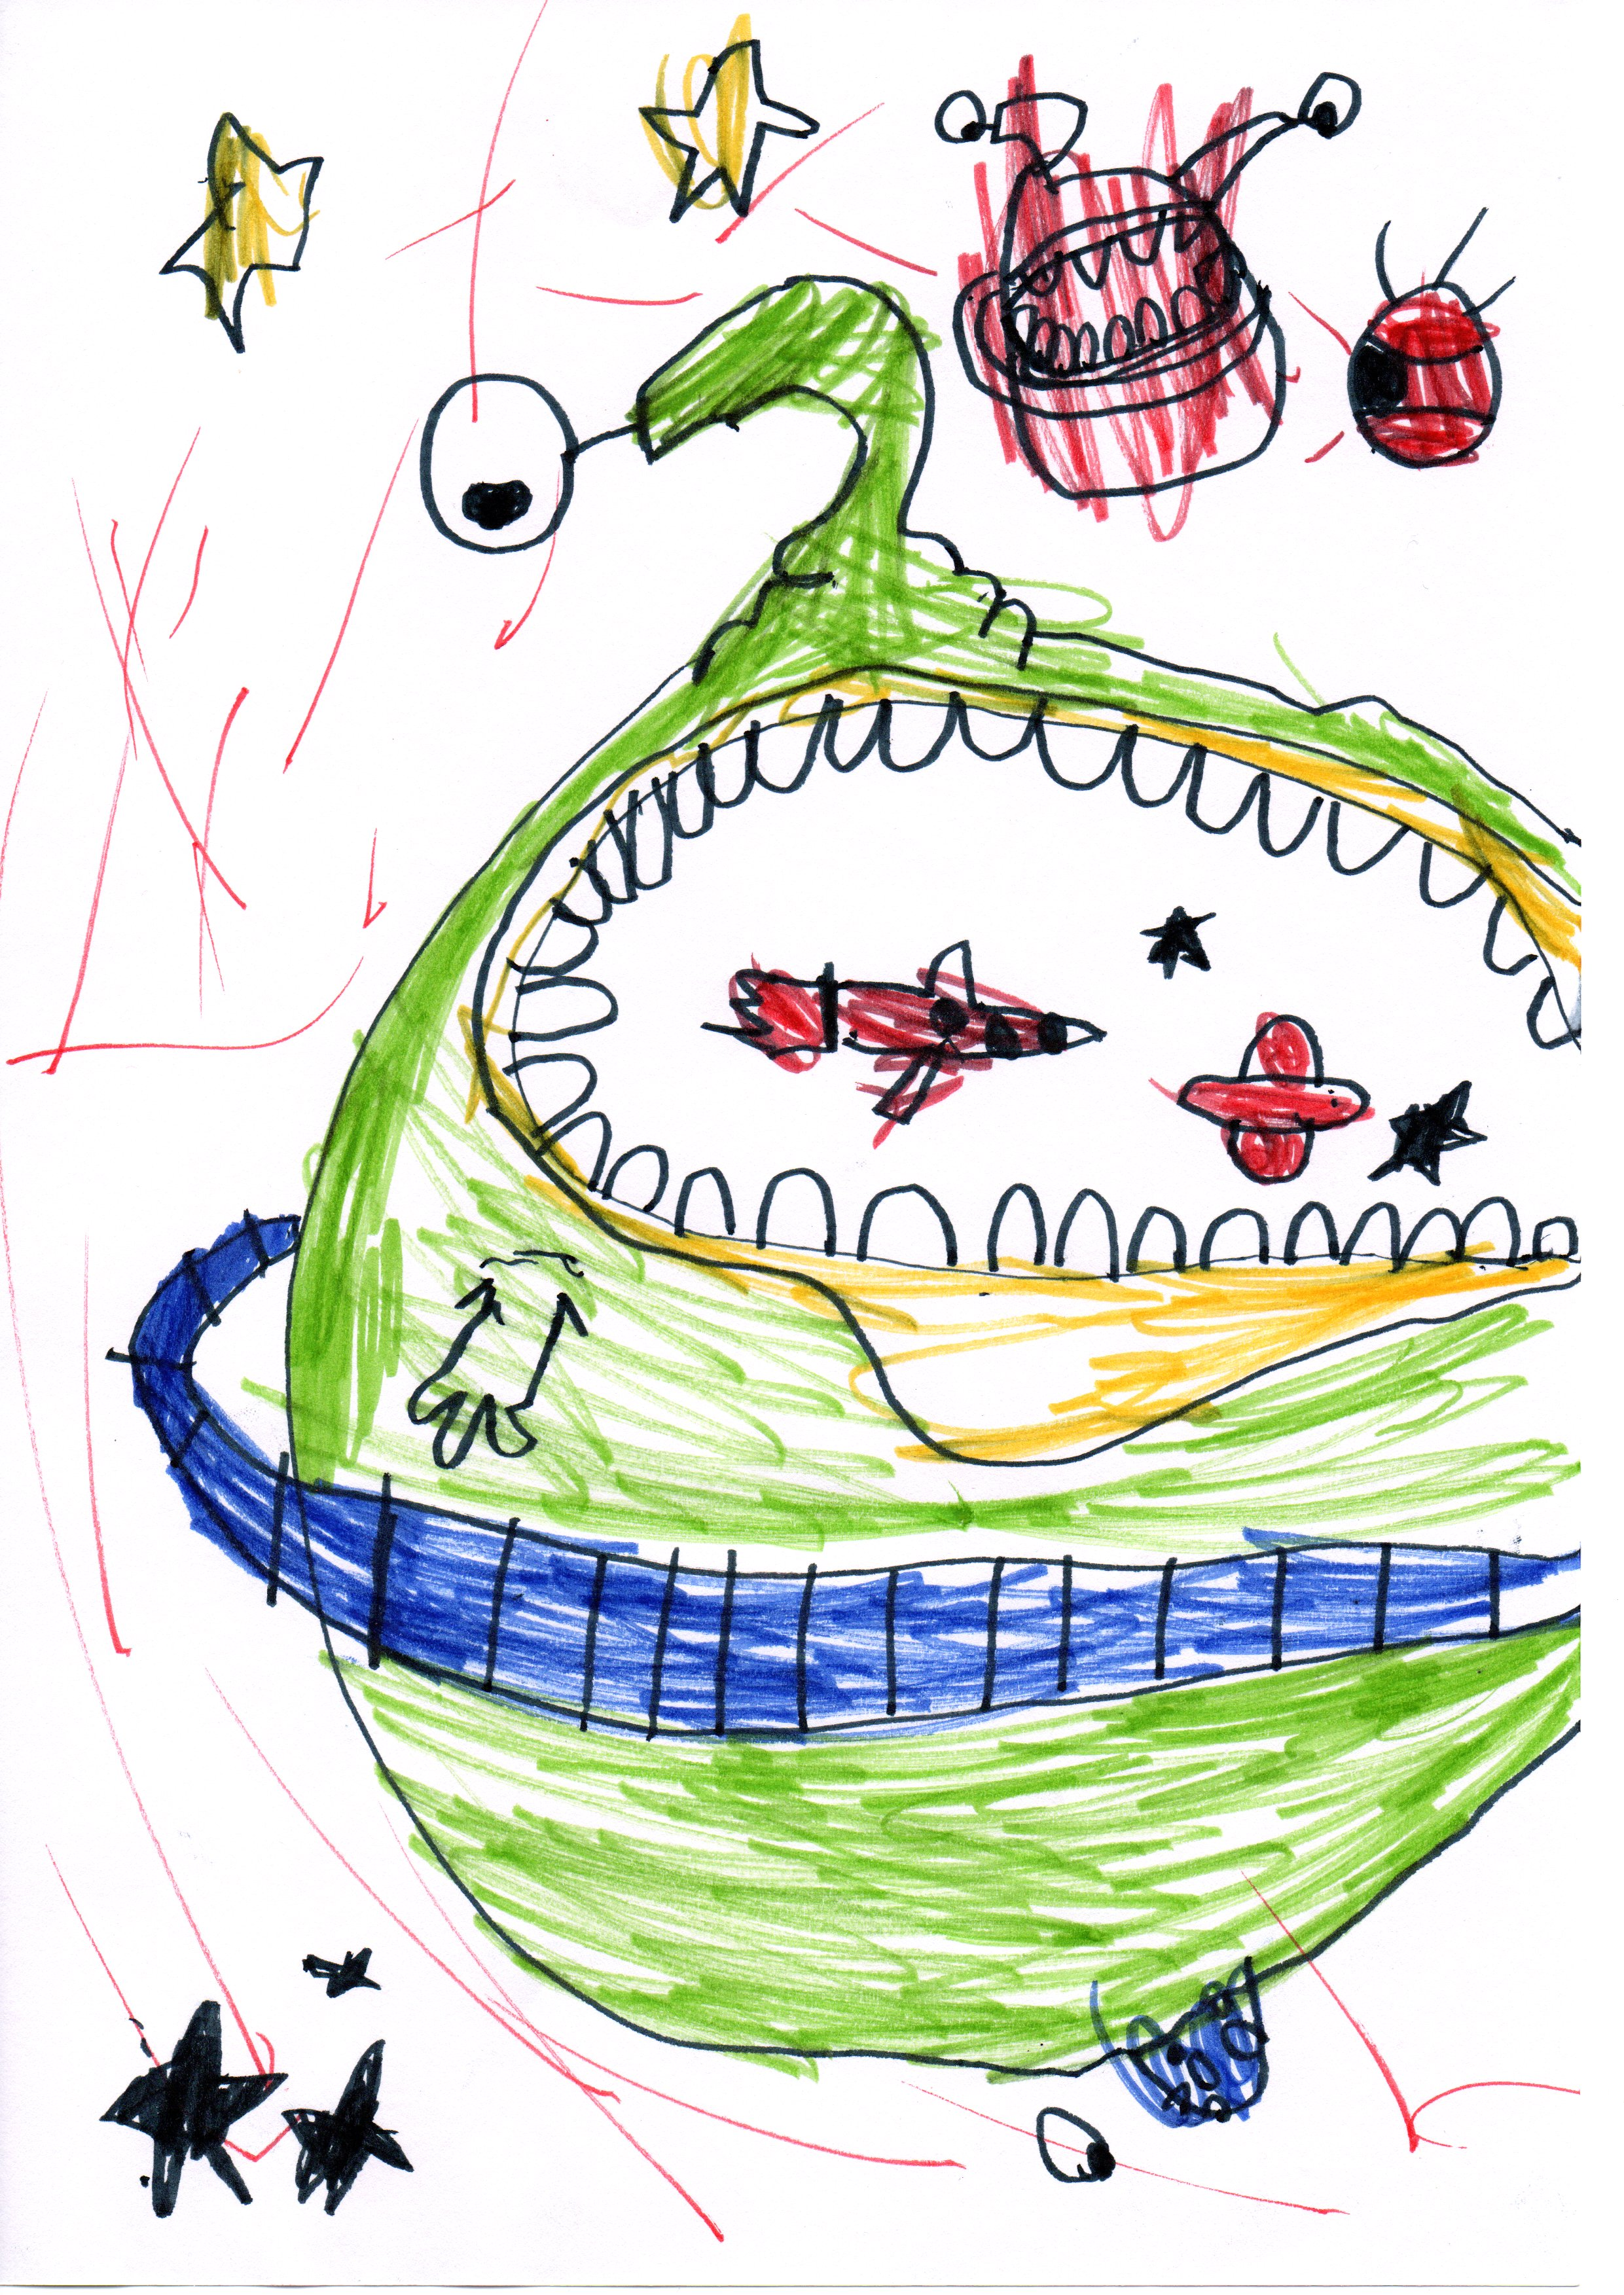
\includegraphics[scale=0.30]{illustrasjoner/Universmonster.jpg}
   \label{Planetmonster}
   \caption{Planetmonster av Helene}
\end{figure}
Hun dro til en stor monsterplanet full av monster.\\
\hfill \\
Planeten var et monster også.\\
\hfill \\
På monster-planeten var det et monster som het Kalle Monsteret.\\
\hfill \\
Kalle monsteret var dronningen til innbyggerne som kaltes Mipmiper.\\ \hfill \\
Kalle monsteret kan kalle på Mipmiperne.\\ \hfill \\

\begin{figure}[H]
    \centering
    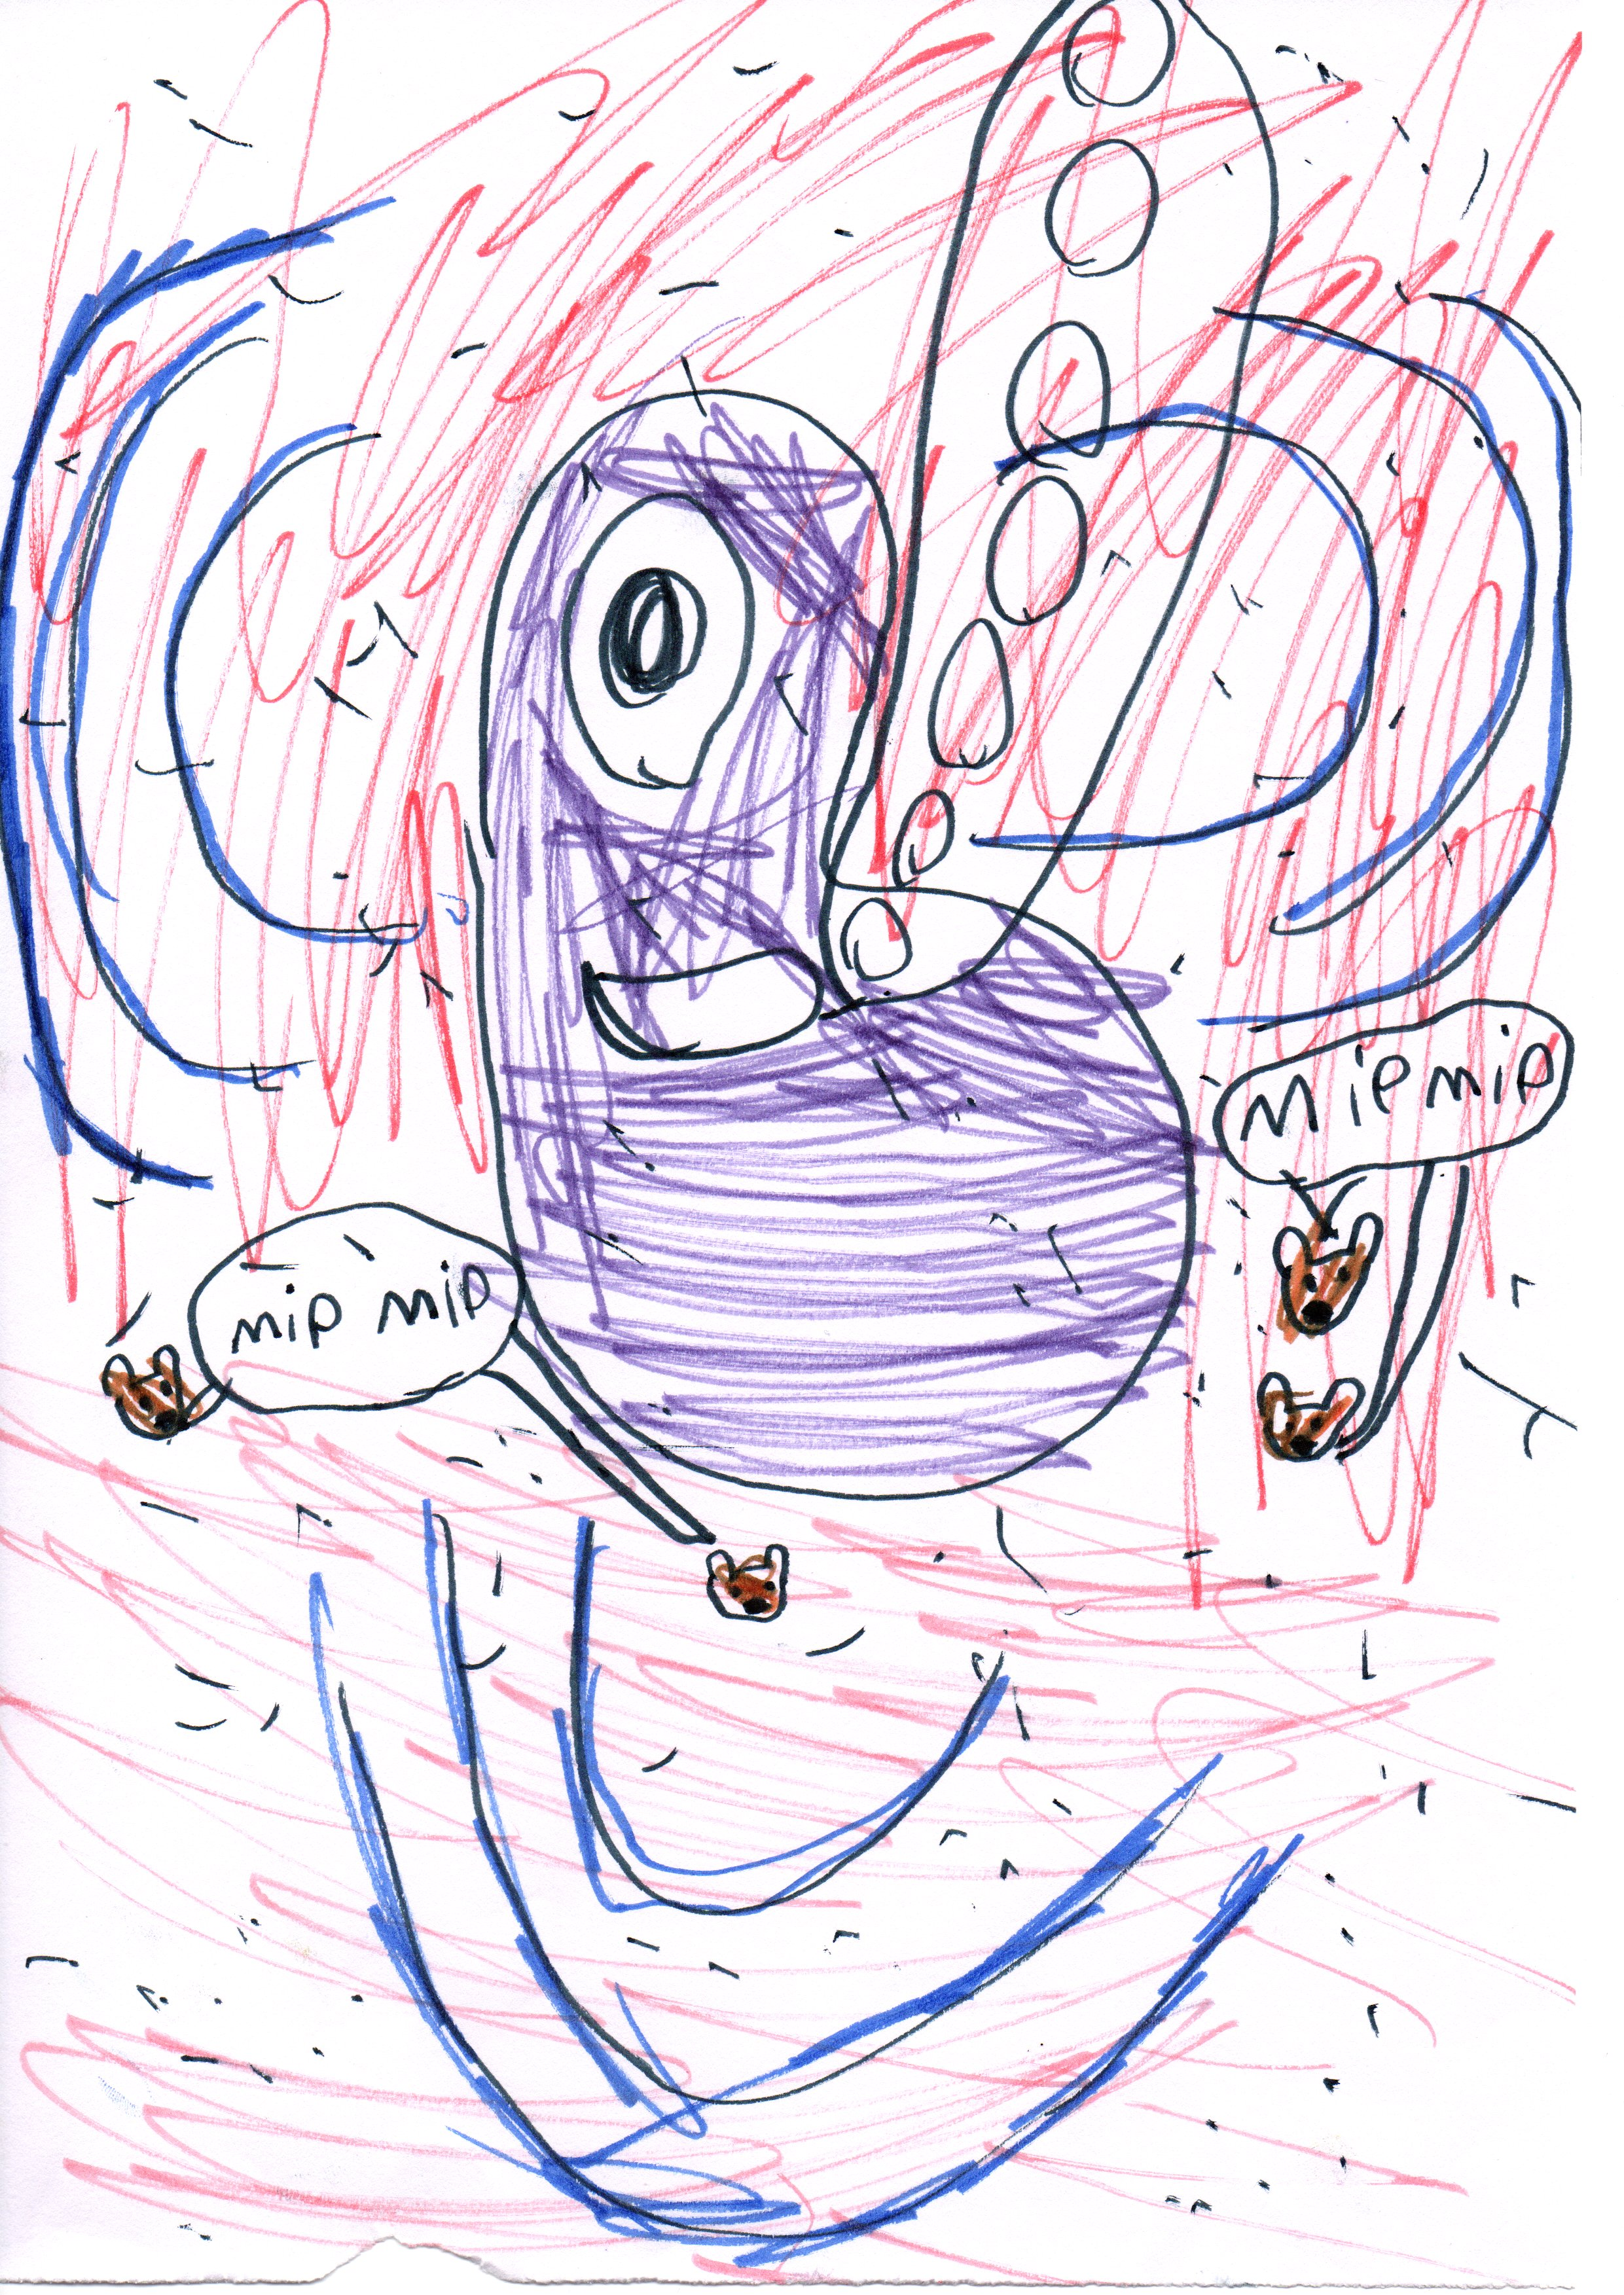
\includegraphics[scale=0.30]{illustrasjoner/kallemonster.jpg}
   \label{kallemonster}
   \caption{Kallemonster av Helene}
Og det var et monster som het Mo monsteret og kalte på Mol.\hfill \newline 

\hfill \newline
\end{figure}
\begin{figure}[H]
    \centering
    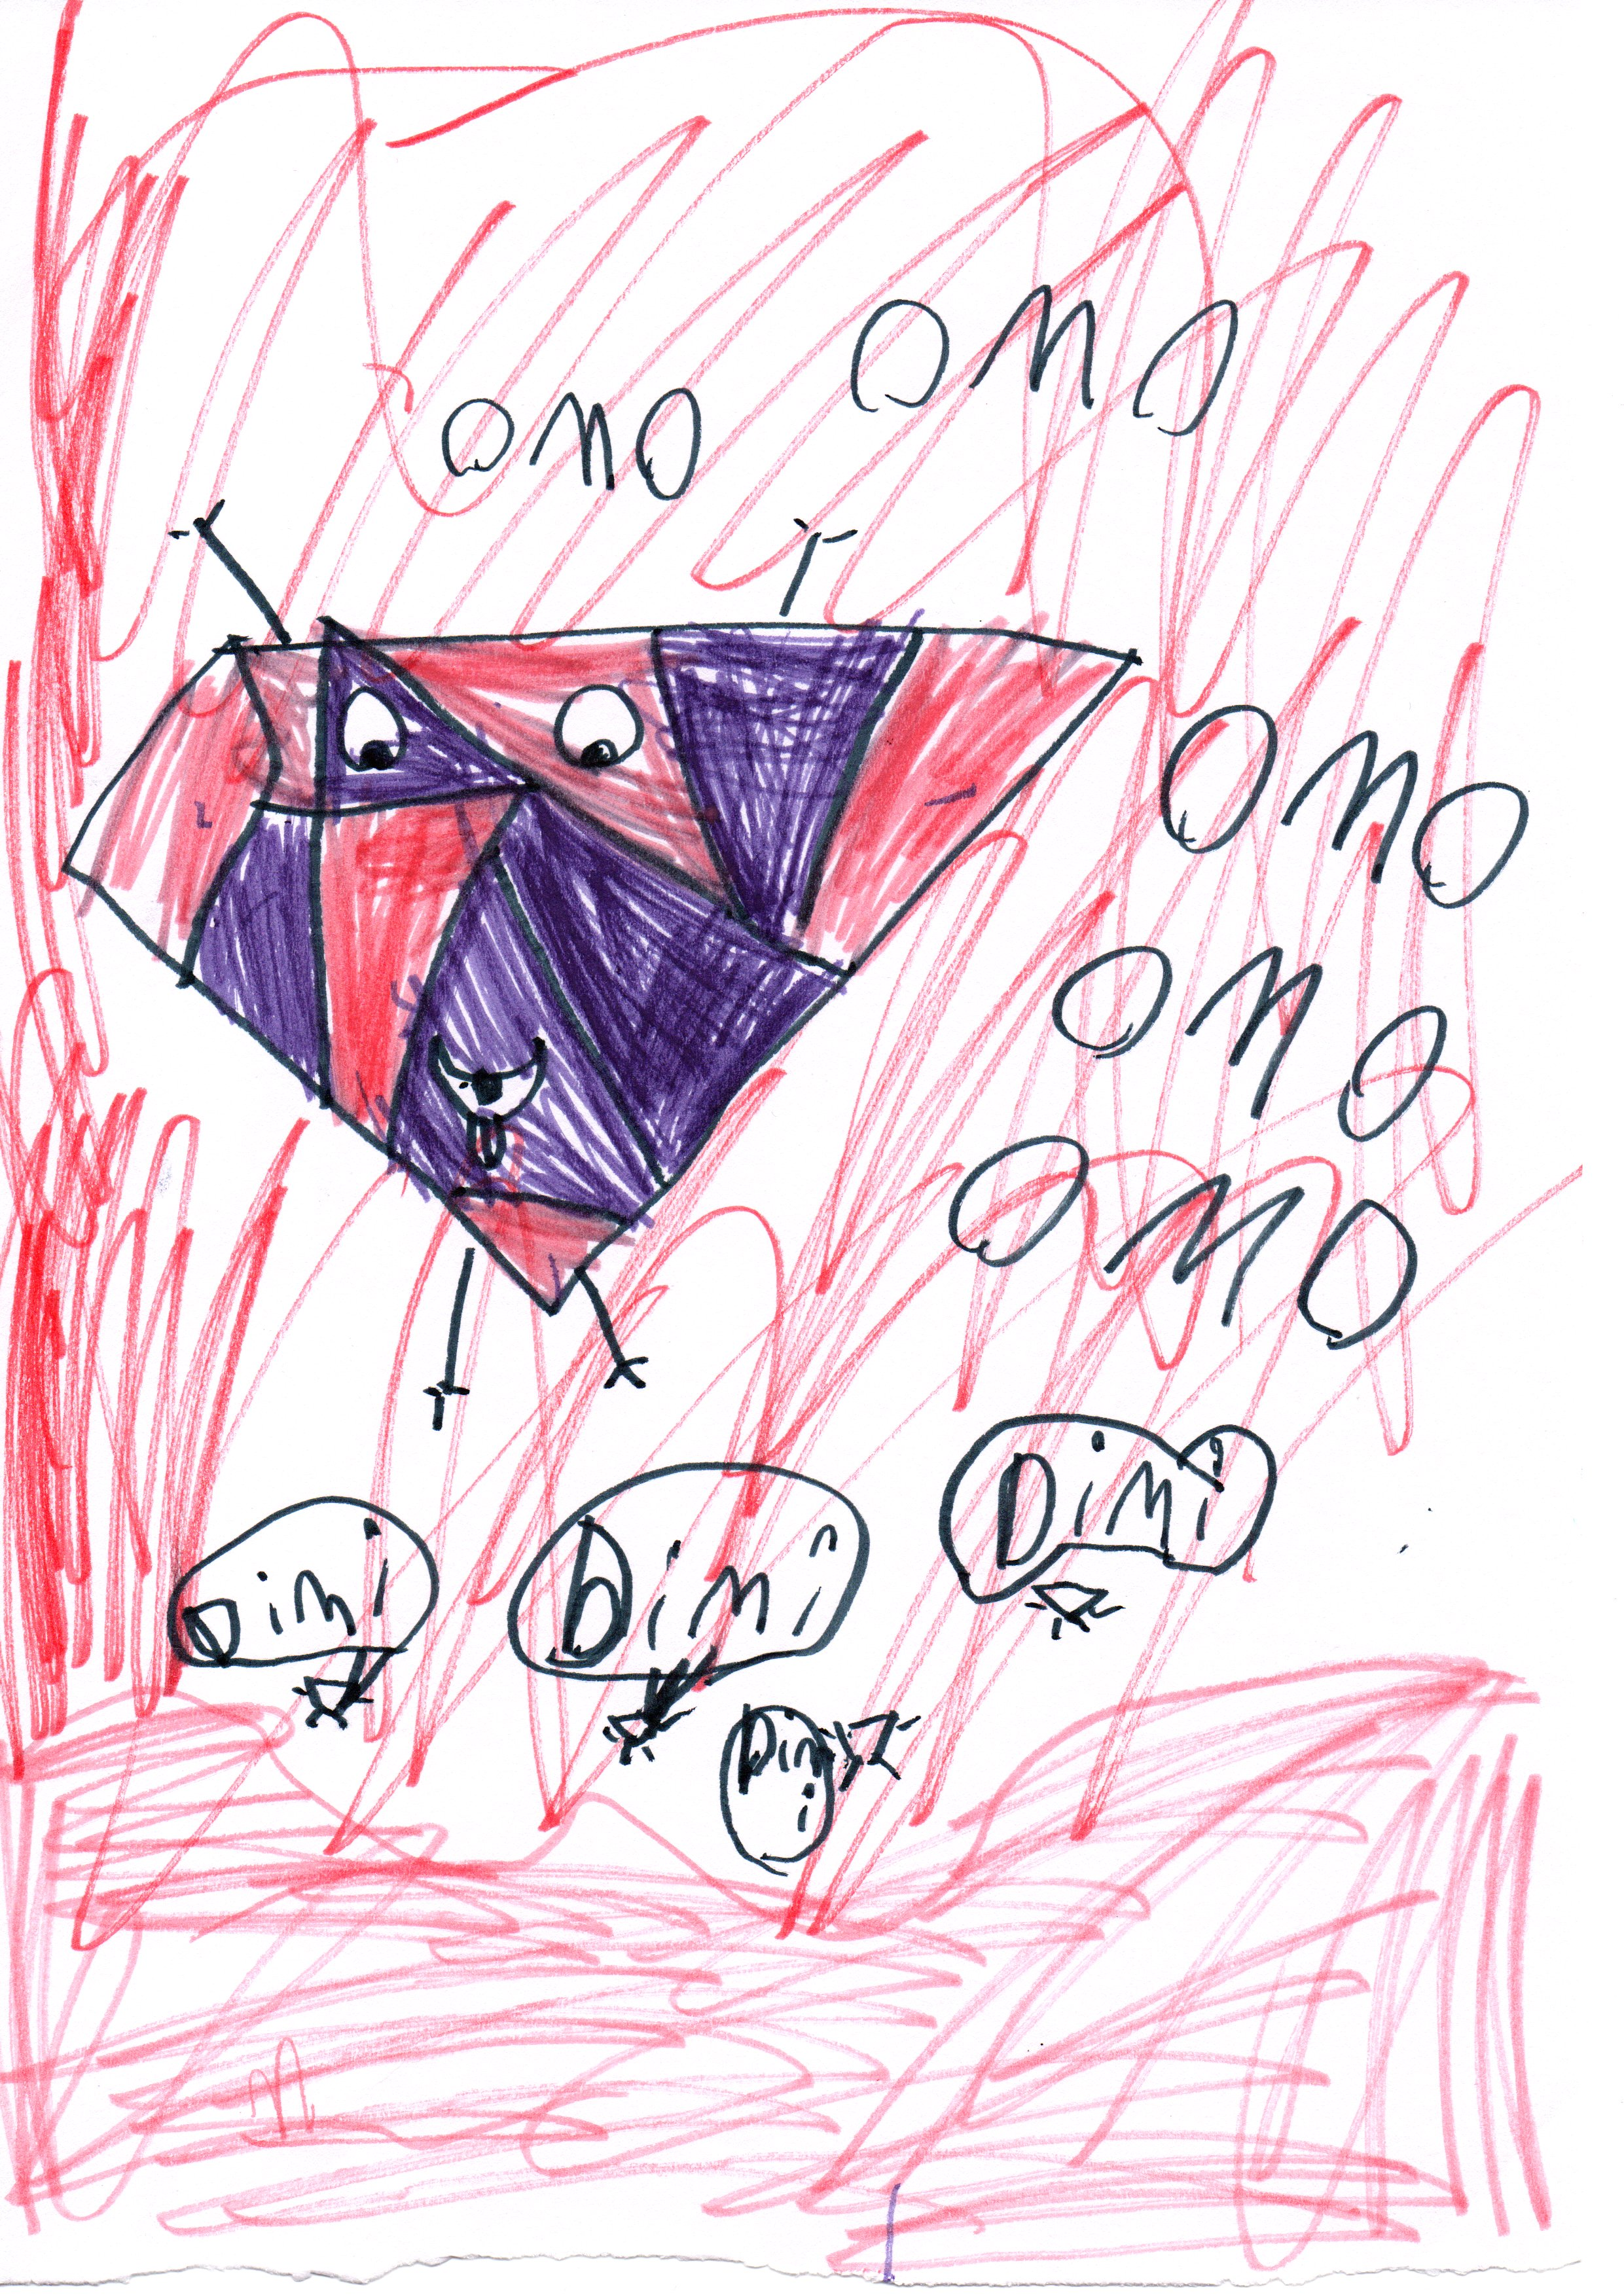
\includegraphics[scale=0.30]{illustrasjoner/omomonster.jpg}
   \label{Omomonster}
   \caption{Omomonster av Helene}
\end{figure}
Det var et monster som het Omo monsteret, og det var det største monsteret og kalte på Dimmi.\\
\hfill \newline 
\newpage
Hun reiste tilbake til Knask og godt, og der sto alle og ventet.\\ \hfill \\
Hun hadde med seg noen bamser og myke ting og litt glitter fra regnbue-planeten og hun fikk med seg noen diamanter til og lage andre og bedre matrealer fra monster-planeten og hun tok med seg noen fine ting fra Ferie-planeten.\\
\hfill \newline
Det kom plutselig et meteor-regn, men hun var alene så hun klarte ikke og stoppe det! \\
Men så kom monsterene og hjalp henne så de klarte og beskytte alle i byen!\\ \hfill \\
Hun var kjempe glad for at monsterene kom og hjalp til med meteorene som kom. Hun var så glad for at hun hadde oppdaget dem, virkelig kjempeglad!!
\begin{figure}[H]
    \centering
    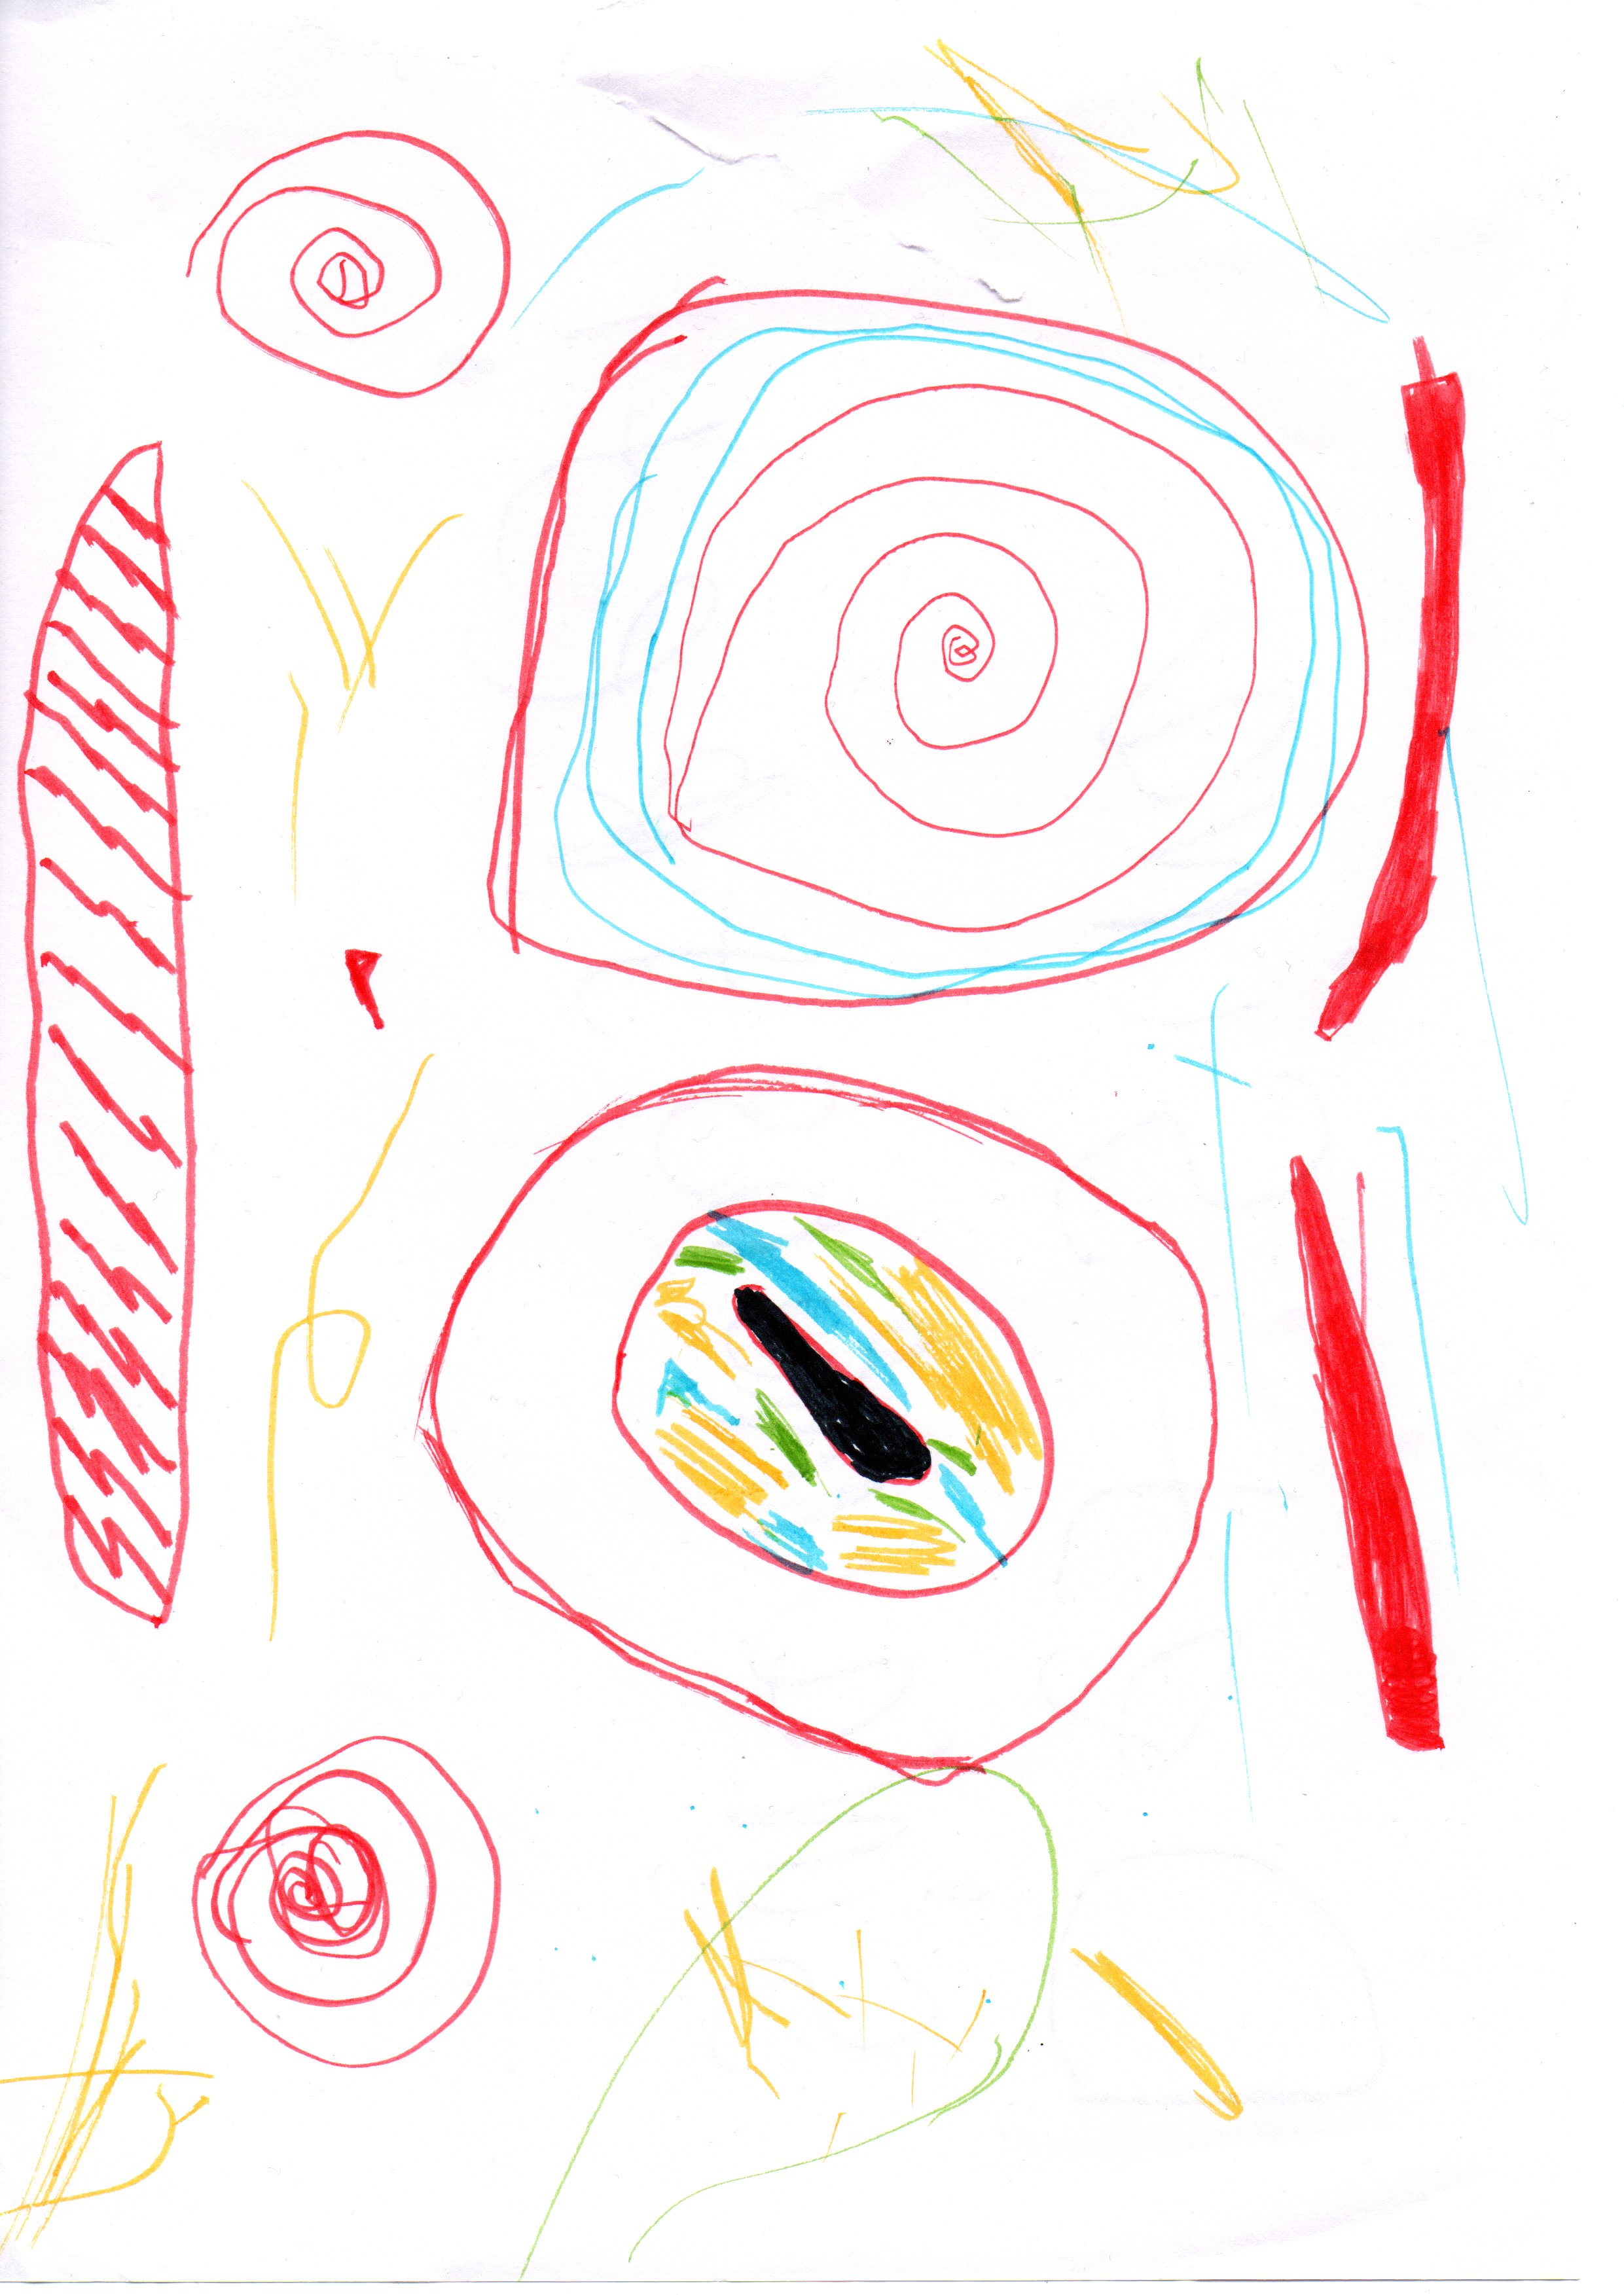
\includegraphics[scale=0.45]{illustrasjoner/Sinnasinnamonsteret.jpg}
   \label{Sinnasinnamonster}
   \caption{Sinnasinnamonster av Helene}
\end{figure}
\begin{figure}[H]
    \centering
    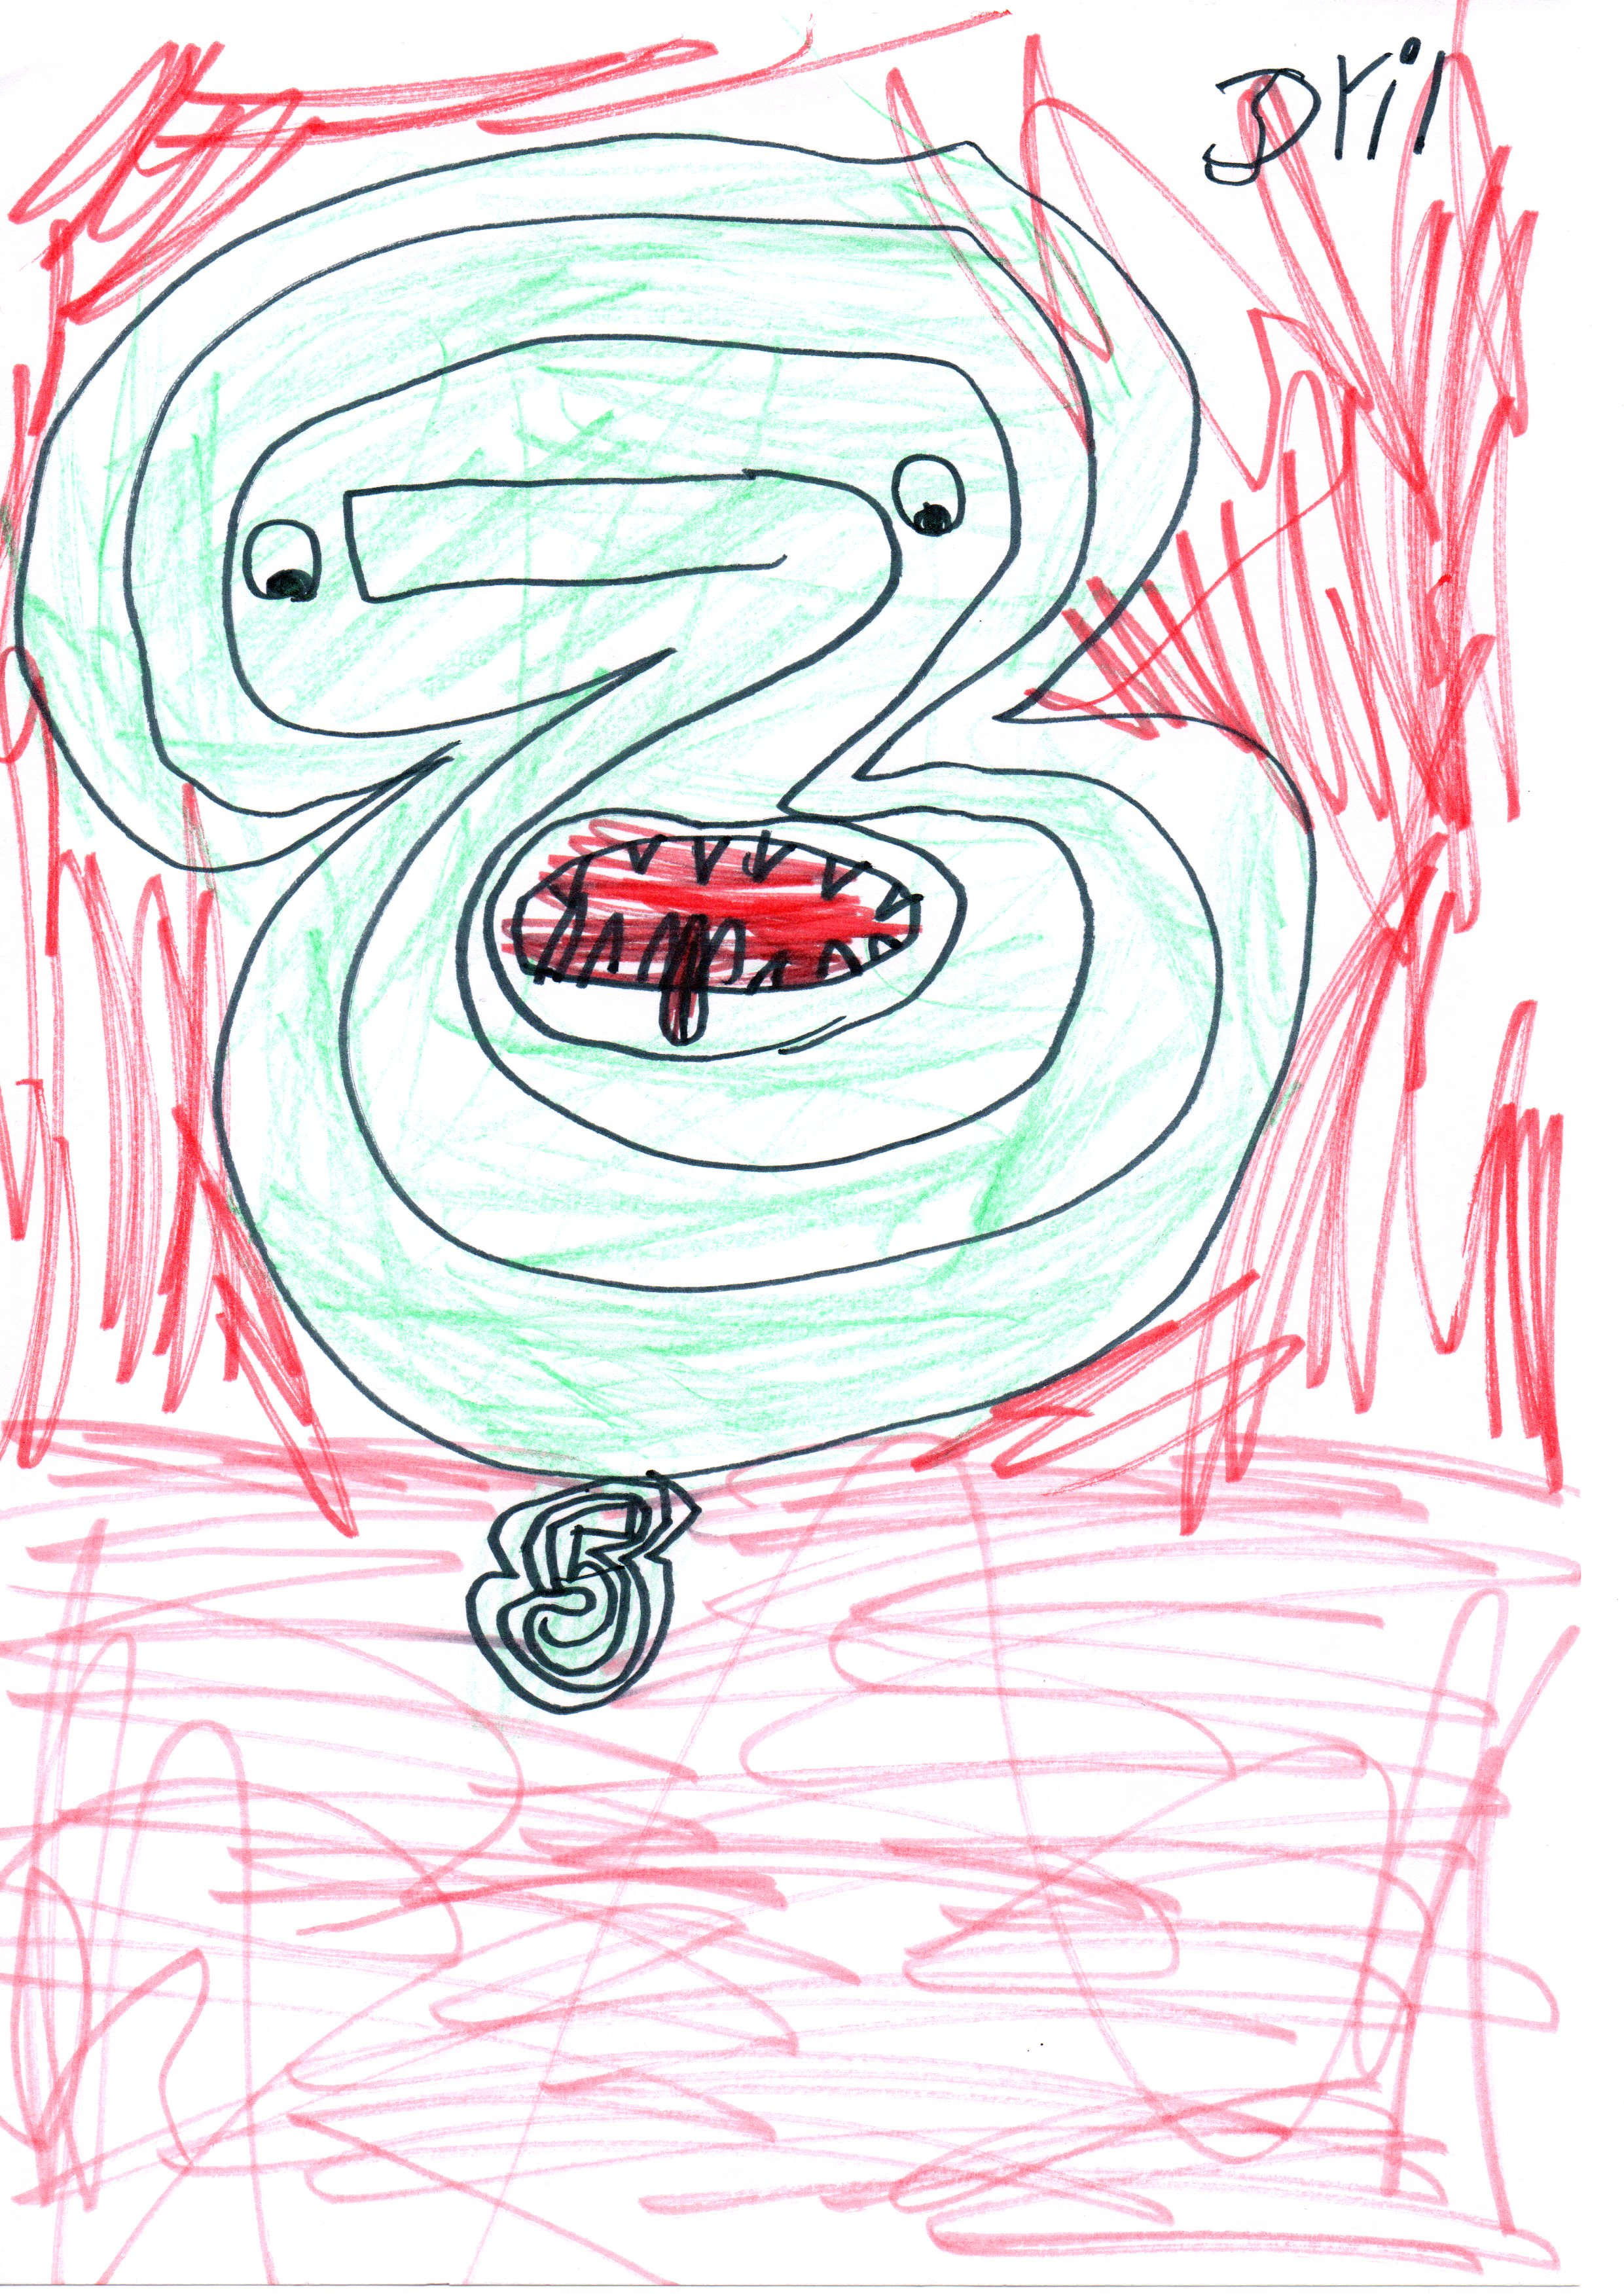
\includegraphics[scale=0.45]{illustrasjoner/groennslangemonster.jpg}
   \label{Grønnslangemonster}
   \caption{Grønnslangemonster av Helene}
\end{figure}
\section{Bortføringene på Knask og godt}
Hun dro til planeten jorden og fortalte alle hva som hadde skjedd men ingen trodde på henne så hun dro for og hente de levende seigmennene men det var ingen der men det var en liten barneseigmann som var der og latet som han var borgemesteren og hadde gullsmykke og han hadde stjelt pengene til alle i byen og sa: \textit{kom slaver}, men det kom ingen slaver. \\
Hun spurte han om hva som hadde skjedd han sa at det var en veldig fin melodi dem ble tiltrukket til og så spurte hun hvordan han ikke ble tiltrukket til melodien han svarte at han hadde headsett og hørte på en annen musikk. Da spurte hun om han viste hvem som hadde spilt musikken. Han viste ikke, men så at seigmennene hadde gått mot et meteorittskip som forsvant så fort som lysets hastighet. Hun spurte hvilken vei dem dro han svarte at skipet gikk til venstre og at hun måtte dra etter det sammen med han så han kunne vise vei. \\
\hfill \newline
Etter hvert så kom de til et sted med rød himmel istedet for et med svart, da skjønte dem at de nærmet seg. \\
Så så de et sted der seigmennene var slaver for aliens! Da skjønte de at dette kunne bli et farlig oppdrag. \\
Hun måtte finne på en god plan, så hun snek seg ned til aliensene.  Aliensene var så mange at mormor måtte få tak i hjelp. Hun dro til monster-planeten, men det var ingen monster der. \\
Det sto et skilt på planeten og der sto det at monsterene var på ferie på Ferie-planeten. Da dro hun til ferie-planeten, men planeten var så stor at det kom til og ta lang tid og finne monsterene. Hun letet og letet, men til 
slutt ga hun opp letingen. \\
Da måtte hun finne ut hva svakheten til aliensene var, så hun dro tilbake til der det var rødt og mørkt. \\
Hun stilte seg intil vinduet og der så hun at konge-alienen var ikke en alien, men en musketur. Musketuren lignet på en hund. Han eller hun latet som han var søt, men nor noen kom og klappet han så ble han et stort og skummelt monster med store hoggtenner og skarpe klør. \\
Hva skulle hun gjøre nå? Men så kom hun på at i det ødelagte romskipet var det gangsterbriller og militær klær og en pistol. Men hvordan skulle hun komme seg tilbake uten og ha blitt sett? Hun sukket lavt for seg. Hva skulle hun gjøre?\\
\hfill \newline
Hun lagde et stort hus. Hun ble der ganske lenge, men til slut hadde hun samlet inn nok info om musketurene. Hun klede seg ut som en alien. Ingen alien merket det. Så hun snek seg in til kongen og sa \textit{noen har stjålet bilen din}.  Plutselig fikk kongen hastverk med å kome seg bilen sin. Da måte mormor jåbe fort da hun hade kommet seg ned til fangehullet.
Og der var ale seigmennene, men vor var vakten som skal pase på fangene? \\
Men der var han! \textit{Han sover}, sa en av seigmennene \textit{og der er nøklene}.\\
Nøklene hang fast i belte hanes, men da tok mormor et sovemidel som hun spraiet onklig got. Hun lirket forsiktig nøkelen ut av beltet til vakten, og fikk ale seigmennene ut. Men hvordan skulle hun få alle tilbake uten å bli opdaget? Så kom på at hun hade røykbomber og røyksyn såm hun kastet til alle seigmennene å så sprag de til romskipet og kom seg trykt jem hun dro til jorda men romskipe kreskja på mars.










%%%%%%%%%%%%%%%%%%%%%%%%%%%%%%%%%%%%%%%%%%
\chapter{Minner og hilsener}
\bigskip
\newpage
\begin{figure}[H]
    \centering
    
\includegraphics[width=1\textwidth]{illustrasjoner/TekstPortrettpsd.jpg}
   \label{Portrett}
\end{figure}
\section{Hilsen fra Jon}
Kjære mamma, \\
Du er litt av en karakter!\\
Jeg husker en episode fra Solvollveien. Det må ha vært før, eller helt i begynnelsen av, barneskolen. Jeg hadde noen kompiser på besøk og viste fram det nye rommet mitt. Det var lekkert med lyst tre på vegger og tak. Du hadde jobbet i ukesvis med å forvandle det store rommet i 2.etg til to barnesoverom, det ene med hems. Jeg synes å huske at Beste var innom og stolt beundret håndverket ditt. Men jeg var ikke stolt, så jeg fortalte kompisene at det var pappa som hadde gjort det. Mammaer skulle liksom ikke fikse og årne… Jeg tror du var skuffet, men du sa ikke så mye.\\
\newline
Det jeg da syntes var pinlig, er jeg nå uendelig stolt av: Denne selvfølgelige selvtilliten din - som får deg til å gå dine egne veier og ikke vike når noen synes du er ukonvensjonell. Du tråkker ufortrødent videre, står i stormen når det blåser og blåser i hva andre mener.  \\
\newline
Jeg tror at dette er noe som har vært ekstremt viktig for oss, alle tre: Ane, Simone og jeg. At du har inspirert oss til å tørre å gjøre ting litt annerledes. Ikke velge helt A4 - selv om vi nå har blitt skremmende etablerte og fått en mengde voksenpoeng alle tre.\\
\newline
Det at du tidlig dro til sjøss har også blitt overført til oss ungene. Det var du som insisterte på at jeg skulle et år på utveksling. Det var den tøffeste utfordringen din 17åringe slubbert til da hadde fått, og noe som har betydd enormt mye. Senere dro du Ane med til Spania og etter det, ble du mammaen til Simone under hennes opphold. Slikt setter ikke bare spor, det har definert oss videre.\\
\newline
En annen ting som gjør meg veldig stolt er hvor mye du bryr deg, og dét har du ikke fra fremmede! Der Mor og Beste alltid hadde en ledig stol for folk som trengte det - både til høytid og hverdag - har du både i arbeid og fritid tatt noen under vingen din. Du begynte tidlig da du ble storesøster for din egen storesøster. Det er vanskelig å si hvordan Britt har hatt det, men det er helt sikkert at du har økt livskvaliteten hennes voldsomt! \\
\newline
For egen del er jeg umåtelig takknemlig for måten du kjempet for meg da jeg slet med dysleksien. Hvor mange personer i hvor mange land du har valgt å forbarme deg over, må foglarna vite. Men det er helt sikkert at vi er mange som er takknemlige! 
Også kommer vi ikke utenom temperamentet. Om det er arv eller miljø skal være usagt, men det er vel ikke noen hemmelighet at flere generasjoner kan ha plukket opp en noe brå stil. Spontanreaksjoner kan få uinnvidde til å skvette, og det som kan virke som en krangel blir av oss sett på som en konstruktiv diskusjon.\\
\newline
På tross av en noe høy temperatur så har jeg alltid følt at det er mulig å komme til deg og prate om alt. Når ting har vært vanskelig har du alltid vært der. Det er noe jeg håper jeg klarer å ta med meg videre, og være en lignende støtte for mine barn.\\
\newline
Veldig glad i deg! \\
Jon


\newpage
\section{Hilsen fra Ane}
Kjæreste mamma,\\
du er og blir en inspirasjon for meg. Tøff, smart og flink, eventyrlysten og god, du har egenskaper som går i arv i barn og barnebarn. \\
Du har en sterk fagbakgrunn som du har brukt til å hjelpe barn og ungdom gjennom en hel karriere. Du har hatt omsorg for alle rundt deg både på og utenfor jobb. Det stoppet heller ikke da du ble pensjonist. \\
Du har flott verdier som rettferdighet, å behandle mennesker med verdighet og respekt for naturen. Dette er jeg veldig stolt av, og du har en fin måte å etterleve disse verdiene på. Du har alltid oppfordret meg, Jon og Simone til å tenke selv og sette spørsmål ved ting. Du engasjerer deg i besteforelderaksjonen og involverer de små til å bli bevisste på hvordan vi kan bli bedre til å ta vare på kloden. Du har en utrolig arbeidsmoral og kapasitet, som noen ganger kan gå litt langt. \\
Du er en fantastisk mormor og farmor og mor, for meg og Jon og ungene, men du tar også vare på resten av slekta. Og ikke nok med det, du har familie i Brasil/England og Indonesia også.\\
Din eventyrlyst, som telegrafist i ungdommen, men også som over snittet reiseglad deretter, har smittet over på meg og Jon. Du har en livsglede og en åpenhet som er fantastisk gøy å være en del av.\\
\begin{figure}[H]
    \centering
    \includegraphics[width=0.9\textwidth]{illustrasjoner/telegrafist.jpg}
   \label{Telegrafist}
\end{figure}

Det å oppleve nye steder med deg er ufarlig og spennende, alt kan bli et eventyr. Som når vi kjørte rundt i Sverige, og kjørte tom tanken, hopp-på-turer til Syden, eller året i Las Palmas. \\
Det har gitt oss en større horisont, for kultur, mat og språk.\\
\newline
Du har alltid fått til alt, om det var å bygge noe, eller å lære noe nytt. Du hopper bare i det, og lander alltid på bena. Jeg er veldig glad for å ha hatt en sånn rollemodell, og for å ha det for mine små. \\
\newline
Varme og omsorg har du også mye av, og det er det som jeg sitter her og tenker på nå. Alle dagene, kveldene og nettene du har vært her for meg når jeg trenger det. De siste årene har det kanskje spesielt vært knyttet til barna. \\
\newline
Tor Håkon sov ikke mye da han var helt nyfødt, fra å ha lest at nyfødte sov 17 timer i døgnet i en babybok, til å få en liten gutt veldig nær kolikk-definisjon, var et sjokk. Han ville ha mat i ett sett, og sov lite. Det var timesvis med skriking, hvor det eneste som kunne hjelpe var å vugge eller trille. Jeg og Per Ole var utslitte, vi prøvde å dele på byrden, men det ble lite hvile. \\ Du stilte opp, fra den første natta på sykehuset og utover. Du vugget og gikk og sang. Timesvis fram og tilbake på stuegulvet og ute. Så jeg fikk sove en stund. Og det var aldri noen klaging fra din munn. Tvert imot var du blid og god, mot ungen og mot meg. Koste og dullet ham, og sa \textit{Gå å lægg dæ, det her orne æ}. Og det gjorde du, alltid.\\
\newline
Disse hvileskjærene har vært gull verdt. Fra en følelse av slit til en tilstand hvor man kan leve litt igjen. Denne følelsesmessige overgangen har lenge fått meg til å tenke på en sang: "What a Diff'rence a Day Made". Selv om sangen egentlig er en kjærlighetssang, fanger den godt hvordan det å ha deg i nærheten føles.\\
\newline
Det viser seg at sangen egentlig er spansk, og det passer jo godt. Den er skrevet av María Grever (14 September 1885 – 15 Desember 1951), som i følge Wikipedia var den første kvinnelige meksikanske komponisten som fikk internasjonal anerkjennelse. I original versjon heter den  "Cuando vuelva a tu lado" ("When I Return to Your Side"). Sangen hadde særskilt suksess på engelsk ved hjelp av Dinah Washingtons flott stemme.\\
\newline
Jeg har tatt meg friheten av å skrive den litt om for anledningen:\\
\newpage
\poemtitle{What a Diff'rence a Day Makes (Ane-versjon)}

\begin{verse}[13em]
What a difference a day made\\
Twenty-four little hours\\
Brought the sun and the flowers\\
Where there used to be rain\\
\bigskip
My yesterday was blue, dear\\
Today I have you, dear\\
My lonely nights are through, dear\\
Since you said you have time\\ 
\bigskip
What a difference a day makes\\
There's a rainbow before me\\
Skies above can't be stormy\\
Since that moment of bliss\\
That bit of rest\\
\bigskip
It's heaven when you\\
Find Trondheim on your menu\\
What a difference a day made\\
And the difference is you\\

\end{verse}

\attrib{María Grever (1885\textendash 1951), med endringer av Ane}

\section{Hilsen fra Simone}
\textbf{Simone’s year in Norway}\\
I am so lucky to treasure many moments with the Dalsen’s family  where I lived for a year. I was there from August 1997 to 1998. During this time I collect several dear moments and several of them include Lisbeth, my host mother!
But we all know that Lisbeth doesn’t like drama, she would rather prefer a good laugh instead. Here are some funny moments I spent with her. Here it goes!

\subsection{Bad deal}
When I first arrived in her house, after having some food, I told Lisbeth that I would do the washing up I liked her food. Little I knew, at the time, about her amazing cooking skills.. so there I was doing the washing up, almost every day.. hahaha
She insisted I did not have to do it, but I happily punished myself for a very good reason – TUSEN TAKK FOR MATEN!!

\subsection{Being late (Following Jon’s habits)}
We were once invited for a dinner in Lisbeth’s friend house (I think her name was Anelise). Dinner was at 5, so I arrived home 16:50 (“just in time, I thought”). But Lisbeth was furious, she said dinner was going to be SERVED at 5 and we should have been there much earlier, so  the dinner have been cancelled/postponed. I had to buy some flowers and apologise to the poor Anelise.
When I told this to my Brazilian parents, they were very proud of Lisbeth, especially because I had been told off, so this story was funny for my parents (but not for me).. hehe

\subsection{Getting on the wrong bus}
***Correction, getting the right bus on the wrong direction..
On my first visit to Naila’s house (who lived in Strinda), I was told to get the bus nr 9 (?)  and  get off on a certain stop.. but the stop never arrived, and there was I, on the last stop, in the middle of nowhere. I then called Lisbeth to pick me up (but I didn’t know where I was). Lucky, out of the blue,  a soul appeared to help me out. 
“I can’t find my way, everything is white, so all streets look THE SAME” hehe

\subsection{Lisbeth crashing on my conversation with Randi}
On Ane’s wedding I was having a chat with Randi, she told me that she had moved house and was trying to explain the location of her new house (on the other hand, I was trying hard to understand with poor Norwegian,  what she was saying ). Then Lisbeth crashed in the conversation and said: “Simone has not clue on what you are talking about” hehe (Imagine my poker face)

\subsection{Friends sleeping over}
I was lucky enough to live in the city centre (in Gyldenløvesgade), all my friends lived far away, so they came to visit very often.
Guilherme (a Brazilian fellow) was living on the country side (in Stjørdal, to be more specific, in fact even we called him Bunad.. hehe). 
He came for a sleep over one night, and Lisbeth said that he could sleep anywhere (she then showed him Jon’s temporary room.. near the kitchen, the one with a bed on the wall and no heating).
Guilherme looked at me and said: “What?? Did she (Lisbeth) just told me to sleep in the FRIDGE? hahahahahaha

\section{Hilsen fra Øivind}
Tell ho tante\\
\newline
Visse medlemmer i Dalsnes-klanen er nok kjent for å være litt i overkant kreative; de vil ofte bygge og skape, reparere (les: ødelegge) og finne ut hvordan ting henger sammen.\\ Det er ingen ende på hvor mange prosjekter de kan ha på gang samtidig, og det er vel ikke til å stikke under en stol at mange av disse prosjektene aldri ender.\\
\newline
Da jeg vokste opp på Mårnes, hendte det seg jo at kreativiteten og skapertrangen til undertegnede kunne bli litt i meste laget for både slekt og naboer. Det var ikke så rent sjelden det ble heftig oppvask (og opprydding) etter diverse prosjekter, men når det hadde roet seg litt hadde mamma ofte en historie om ulike episoder fra Kvæfjord, og de som vokste opp på Dalsnes… og det kunne være en god trøst å få bekreftet at noen hadde gjort lignende sprell før meg.\\
\newline
En av historiene som ble gikk igjen, var om unge Lisbeth. Og ett av hennes prosjekter. \\
Det skal sies; detaljene i historien har blitt noe utvasket med tiden, siden det naturlig nok er en stund siden sist den ble gjenfortalt. Men dette er jo i seg selv en god grunn til å utøve litt kunstnerisk frihet og tilføre litt farge til historien.\\
\newline
\textit{Beste} som vi barnebarna kalte han, eller \textit{Velle} som han ellers var kjent som; var en dyktig håndverker og møbelsnekker, og en inspirasjon for mange av oss etterkommere.\\På et tidspunkt mens Dalsnes-barna fremdeles var barn, og heimen på Dalsnes kunne trenge en sårt etterlengtet oppgradering av stuebordet, var Beste så heldig at han fikk fatt i et plateemne i Teak, av fantastisk kvalitet. Dette skulle det bli flott stuebord av!\\
Plateemnet ble satt på stabburet slik at det var klart til utforming og bearbeiding. En så alvorlig oppgave som å designe og lage et stuebord, kan ikke tas lett på. Det er en prosess som krever planlegging og bearbeiding gjennom utallige små grå, før det endelig havner på saga. Platen fikk stå der til planen var klar, og tiden strakk til!\\
\newline
Det Beste ikke hadde tenkt på, er at kreative barn alltid har åpne øyne og er på konstant jakt etter idéer, prosjekter, inspirerende emner… - Og emner, materialer og verktøy er alltid det som mangler, en plankebit som er lang nok, flere bord som er like, for ikke å snakke om plater og store emner. Det finner man ikke i hvilken som helst plankehaug! \\
\newline
Naturlig nok fant unge Lisbeth dette høvelige bordemnet, og man skulle bare ønske man kunne få vite hvilke planer og idéer som ble fremkalt og forkastet før den endelige planen åpenbarte seg – dette stykket blytungt treverk måtte være det optimale emnet for å skape tidenes raskeste kjelke! En egen kjelke, som hun hadde ønsket seg så lenge, og jeg velger å tro at lang tids dagdrømming om hvordan denne kjelken skulle se ut, hadde båret frukter. \\Planen var klar! Unge Lisbeth var klar! Og snart skulle kjelken være klar!\\
\newline
Så vidt jeg kan kan huske, er intet fortalt om hvilke kjøreegenskaper denne kjelken hadde, ei heller om hvilke fartsrekorder som ble satt. Ble prosjekt kjelke i det hele tatt ferdigstilt? – Til tross for iherdig detektivarbeid, har vi ikke lykkes i å finne flere detaljer eller dokumentasjon om historien. \\
\newline
Og de som kjente Beste, Velle; visste jo godt at han ikke alltid var veldig mild og overbærende, det kunne gå ei kule varmt når han irettesatte oss. Han var streng, sterk, og han kunne nok fått både konger og keisere til å krympe seg i skam når han fortalte hvor skapet skulle stå. \\
\newline 
Nettopp derfor var det vel at en hel familie, for ikke å snakke om ei heil grend, var i sjokk når de hørte at selveste Velle ikke hadde så mye han ville si om denne saken. Ingen heftige reprimander, ingen husarrest, unge Lisbeth ble ikke en gang sendt i seng uten kveldsmat! \\
\newline 
Blandede følelser kjenner vi nok alle til fra ulike hendelser, men jeg tenker at stoltheten Beste hadde til denne egenrådige, smarte og sterke dattera må ha vært ganske sterk når han innså hva hun hadde gjort og hva hun ville skape med dette emnet som egentlig skulle bli familiens nye stuebord. \\
\newline
Denne historien sier ikke så rent lite om personligheten til denne unge jenta, denne fantastiske damen som nå har fylt 70 år; om kreativitet, skapertrang, iherdighet… og MOT!\\
\newline
Gratulerer så hjerteligst med de 70, tante. Vi er heldige som har deg som tante og tidvis «reserve-bestemor» i tunge tider. Vi setter umåtelig pris på din rolle som \textit{senter} i Dalsnes-klanen, den som kaller inn til sommertreff og holder oss sammen. \\
\newline

Beste hilsener,\\
Øivind\\
Cecilie, Magnus og Sofie

\newpage
\section{Hilsen fra Ida}
Biltur fra Dalsnes til Harstad i gamle \textit{Svarten}.\\
Mor Oline og tante Lisbeth i forsetet, og mamma Kristin og Ida i baksetet. På hattehylla den fiiiine hunden med dinglehodet.\\
\newline
Søstrene har funnet et tema å dissekere, så etter 7 min biltur ber Mor om å bli satt av for å slippe å høre på kranglinga, hvorpå svaret helt klart er at de jo bare diskuterer. Men det blir litt roligere i bilen. \\
\newline
Nesten 20 år senere biltur med 3 av damene fra Budapest til Balaton. Vin, sightseeing, samtaler og kos, og vonde bein som et par påler ned i et iskaldt basseng $\heartsuit$ \\
To blad Fredriksen-søstre med sterke meninger, men alltid gode venner. Ei fantastisk søster for mamma og tante for meg, som det alltid har vært og er godt å ha, som venn, samtalepartner, støtte i tunge og gode tider, eller med seg i skyttergrava. Og perfekt som reservebestemor for mine gull $\heartsuit$ \\
\newline 
Jeg setter utrolig stor pris på deg, tante Lisbeth! \\
Gratulerer med de 70, håper det blir mange til med fine stunder og gode prater. \\
Glad i deg $\heartsuit$ \\


\section{Hilsen fra Club 75}
\begin{centering}
Mange gratulasjoner til en sprek 70 åring\\ 
fra alle oss i CLUB 75 !\\ \hfill \\
Fortsett å bestige fjell på Gran Kanary,\\
så kan vi ta oss av strandlivet!\\
\end{centering}
\begin{figure}[H]
    \centering
    
\includegraphics[width=0.9\textwidth]{illustrasjoner/Underskrifter.png}
   \label{Hilsen}
\end{figure}



\section{Hilsen fra Sylvi}
\begin{figure}[H]
    \centering
    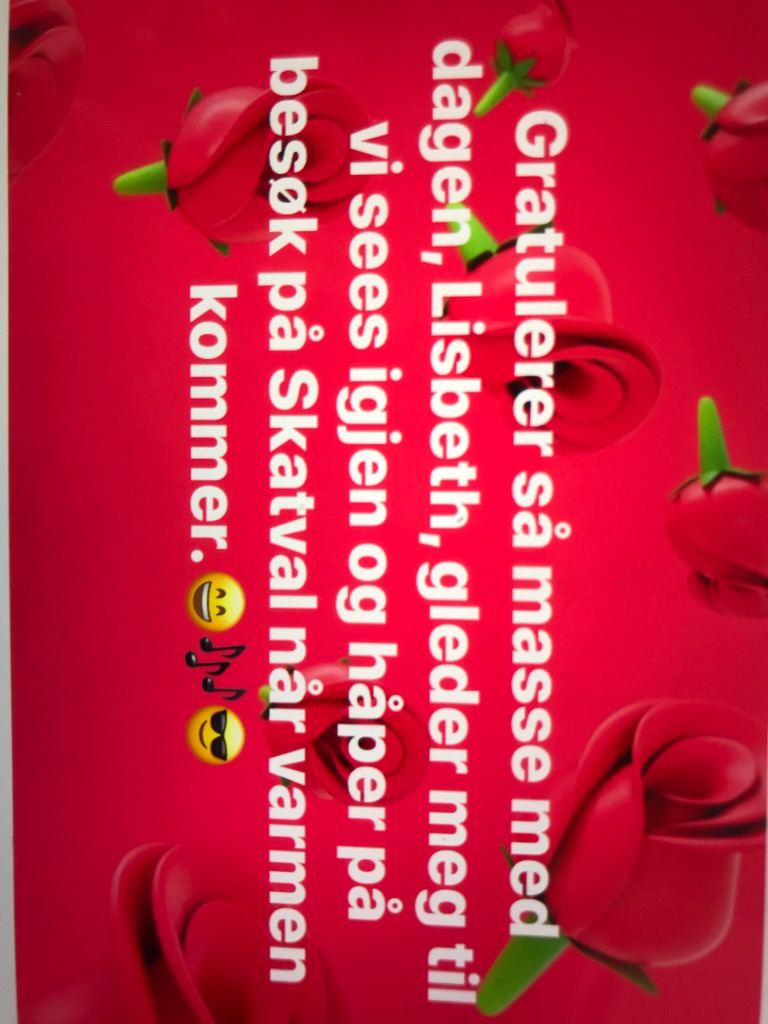
\includegraphics[width=0.75\textwidth, angle=90]{illustrasjoner/Sylvihilsen.jpg}
   \label{Hilsen}
\end{figure}
\section{Hilsen fra Ingerid}
\begin{figure}[H]
    \centering
    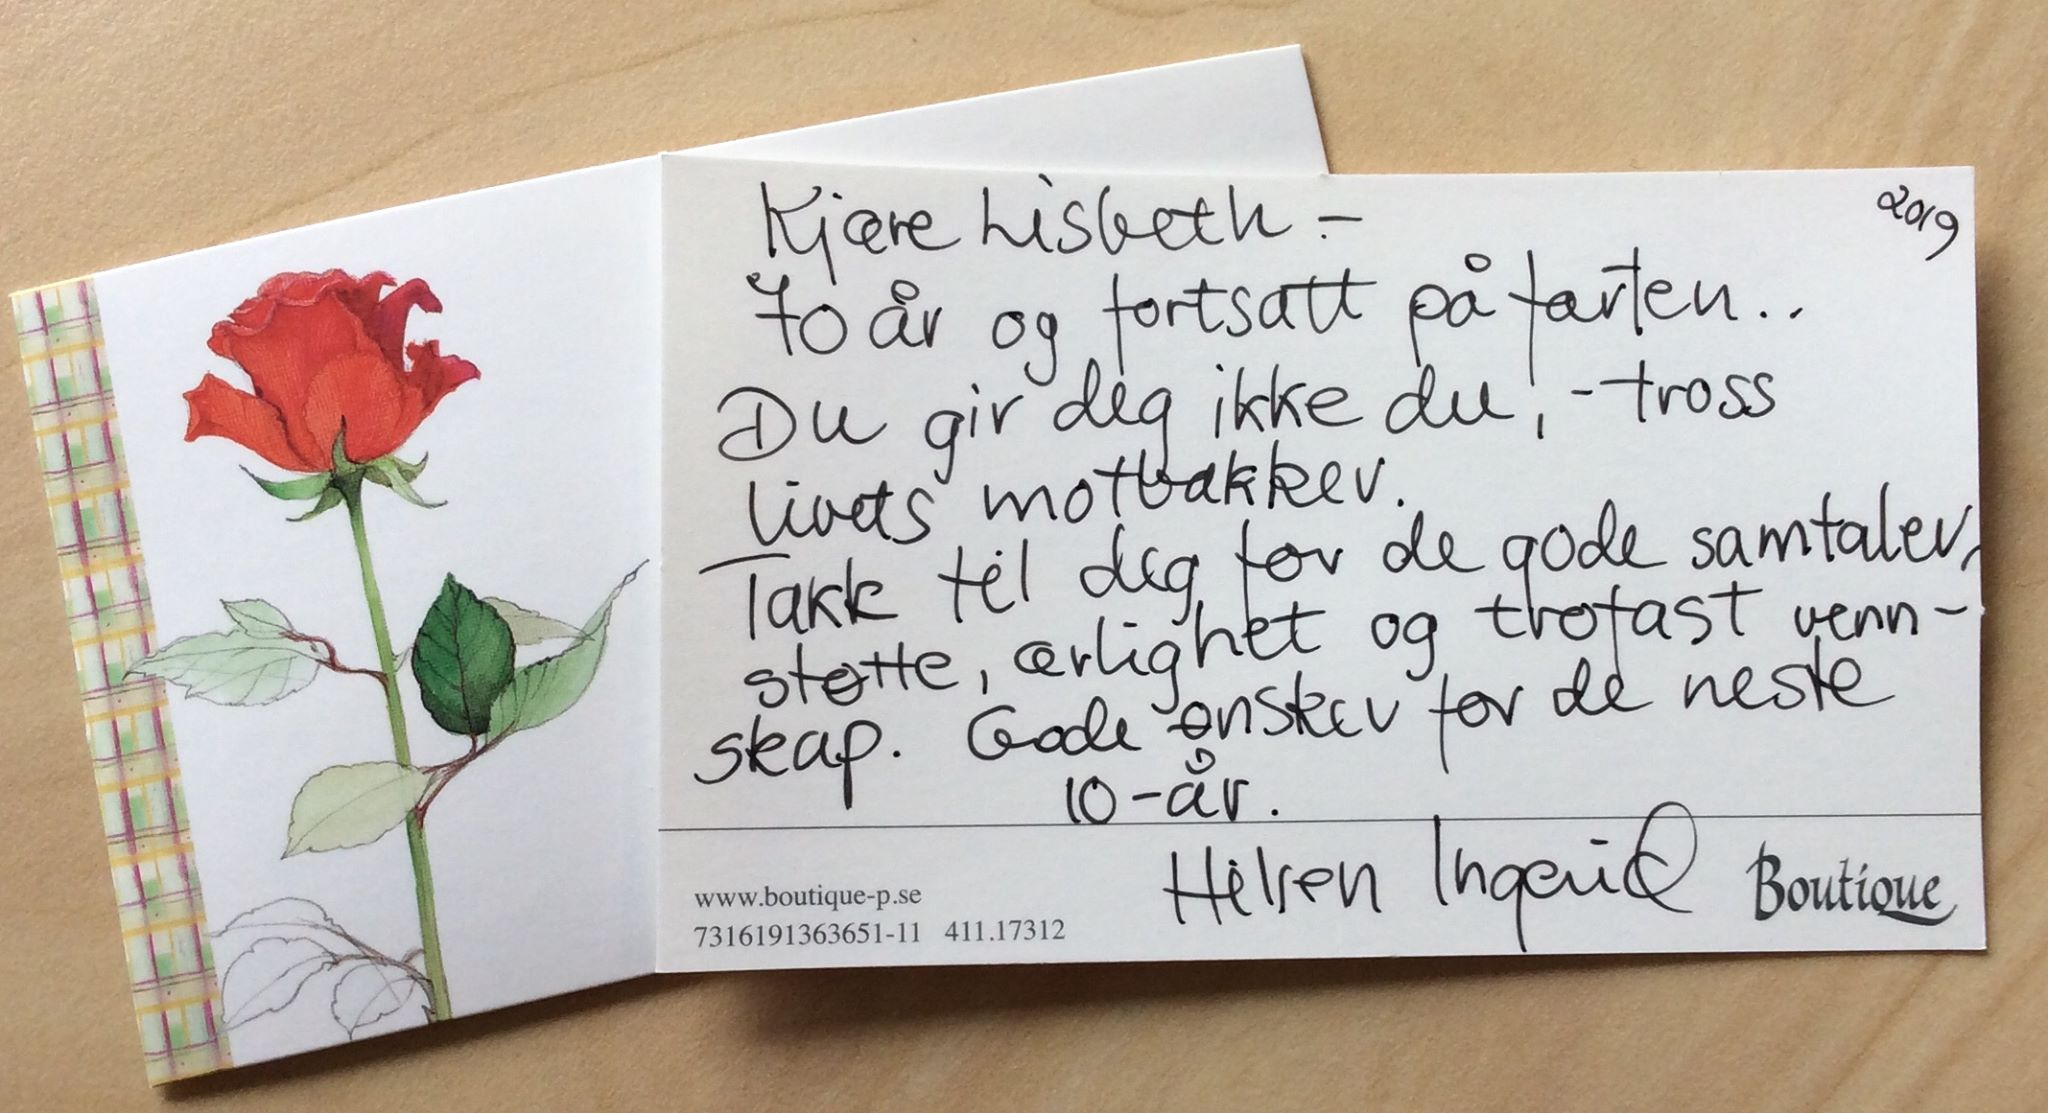
\includegraphics[width=1\textwidth]{illustrasjoner/Ingerid.jpg}
   \label{Hilsen}
\end{figure}
\section{Hilsen fra Lise}
\begin{centering}
Kjære, kjære Lisbeth\\
Du er tidenes venninne\\
Hilsen Lise
\end{centering}

%\begin{figure}[ht]
%    \centering
%    \includegraphics[width=1\textwidth]{Bryllupssang_fra_Erik.jpg}
%   \label{bryllupssang}
%    \caption{Brylllupssang skrevet av Gerds lillebror Erik}
%\end{figure}


\end{document}
